%\documentclass[preprint,3p,times,twocolumn]{elsarticle}
\documentclass[review,3p,times]{elsarticle}
\usepackage{amssymb}
\usepackage{amsmath}
\usepackage{graphicx}
\usepackage{bm}
\usepackage{yhmath}
\usepackage{subfig}
\usepackage{multirow}
\usepackage{cleveref}
\usepackage{xcolor}
\definecolor{Rev1}{rgb}{0,0,0}
\definecolor{Rev2}{rgb}{0,0,255}
\usepackage{subdepth}
%\usepackage[nomarkers,lists]{endfloat}

\def\pp#1#2{\frac{\partial #1}{\partial #2}}

\biboptions{comma,sort&compress}

\journal{Combustion and Flame}

\makeatletter
\def\@author#1{\g@addto@macro\elsauthors{\normalsize%
    \def\baselinestretch{1}%
    \upshape\authorsep#1\unskip\textsuperscript{%
      \ifx\@fnmark\@empty\else\unskip\sep\@fnmark\let\sep=,\fi
      \ifx\@corref\@empty\else\unskip\sep\@corref\let\sep=,\fi
      }%
    \def\authorsep{\unskip,\space}%
    \global\let\@fnmark\@empty
    \global\let\@corref\@empty  %% Added
    \global\let\sep\@empty}%
    \@eadauthor={#1}
}
\makeatother

\begin{document}

\begin{frontmatter}

\title{Ignition and extinction of strained nonpremixed cool flames at elevated pressures}

\author{Sili~Deng}
\author{Dong~Han\fnref{fn}}
\author{Chung K.~Law\corref{cor}}
\cortext[cor]{Corresponding author: cklaw@princeton.edu}
\fntext[fn]{Permanent address: Key Laboratory of Power Machinery and Engineering, Ministry of Education, Shanghai Jiao Tong University, Shanghai 200240, China.}

\address{Department of Mechanical and Aerospace Engineering, Princeton University, Princeton, NJ 08544, USA}

\begin{abstract}

Cool flames, governed by low-temperature chemistry, are closely related to engine knock.  Since the low-temperature chemical kinetics is promoted at elevated pressures, the ignition and extinction of nonpremixed cool flame at elevated pressures were experimentally and computationally investigated herein in the counterflow.  Specifically, the hysteretic ignition and extinction behavior of the nonpremixed cool flame was for the first time observed and quantified.  S-curve analysis was conducted to demonstrate the thermal and chemical structure of the cool flame and to elucidate the dominant chemical pathways during the ignition and extinction processes.  The dominant low-temperature chemical reactions shift from those responsible for radical runaway to exothermic reactions that sustain the cool flame.  Increasing the ambient pressure and/or the oxygen concentration in the oxidizer stream promote the heat release from the cool flame, and hence, result in an extended hysteresis temperature window between ignition and extinction.  It is further noted that while the observed cool flame ignition temperatures were well predicted by computation, significant discrepancies existed for the extinction temperatures based on the well-adopted reaction mechanism used.  Possible reasons were discussed to facilitate further cool flame studies and the development of the low-temperature chemistry.

\end{abstract}

\begin{keyword} 
Cool flame \sep Low-temperature chemistry \sep Ignition and extinction \sep Elevated pressure \sep Nonpremixed counterflow 
\end{keyword}

\end{frontmatter}


%\clearpage % For word count
%==============================================================

\section{Introduction}

Cool flames, first reported in 1817~\cite{davy17}, are controlled by low-temperature chemical kinetics that have been extensively studied ever since~\cite{griffiths87}.  \textcolor{Rev1}{Such low-temperature chemistry is ubiquitous for most large hydrocarbon fuels and has been shown to be related to the negative temperature coefficient (NTC) phenomenon observed in autoignition processes~\cite{leppard90,ciezki93} and engine knocks~\cite{griffiths02}.  The fundamental understanding of low-temperature chemistry and cool flame dynamics can also be important for combustion phasing control in the recent development of homogeneous charge compression ignition (HCCI) engines~\cite{kong01,lu11} and reactivity controlled compression ignition (RCCI)~\cite{kokjohn11} engines.}

\textcolor{Rev1}{Besides the potential utilization in engines, the dynamics of the cool flame are of fundamental interest.  Cool flames and the NTC phenomena have been mostly observed in homogeneous systems such as rapid compression machines~\cite{griffiths02b,silke05,di14}, shock tubes~\cite{ciezki93,vasu08,herzler05}, flow reactors~\cite{koert94,curran00} and stirred reactors~\cite{dagaut95,kikui15}.}  Without the complexity of inhomogeneity and transport, low-temperature chemical kinetics can be studied in these systems for chemical model development.  However, in practical combustors such as the diesel and gasoline direct injection (GDI) engines, combustion processes are governed by both transport and chemical kinetics.  For such conditions, the characteristic mixing time scales can be comparable to the chemical reaction time scales, and the convective-diffusive processes may affect the initiation and sustenance of cool flames.

Recognizing that the inevitable presence of nonuniformities in practical combustion systems requires consideration of the coupled effects of chemistry and transport on cool flames, cool flames in nonpremixed systems have been recently studied in the counterflow~\cite{law12,zhao13,deng14,won15} and microgravity droplet combustion~\cite{nayagam12,farouk15,nayagam15}.  In particular, Law and Zhao~\cite{law12} and Zhao and Law~\cite{zhao13} numerically investigated the nonpremixed counterflow cool flame of $n$-heptane, and identified the existence of a secondary S-curve dominated by low-temperature chemistry at low strain rates and/or high pressures.  This secondary S-curve is grafted onto the lower branch of the primary S-curve and has its own ignition and extinction turning points.  Experimentally, nonpremixed cool flames were observed in the counterflow at atmospheric pressure~\cite{deng14}, including those employing a reactivity promoter~\cite{won15,ju16}.  The ignition temperature of dimethyl ether (DME) was quantified with infrared imaging~\cite{deng14}, and was found to increase with increasing strain rate but was insensitive to the DME concentration in the fuel stream.  In microgravity droplet combustion, it was found that the visible flame of large $n$-heptane, $n$-octane, and $n$-decane droplets could transit to a quasi-steady low-temperature burning mode after extinction of the hot flame due to radiation, suggesting the existence of steady droplet burning sustained by a cool flame~\cite{nayagam15}.  

Since low-temperature chemistry is more pronounced at elevated pressures, which for example could affect flame stabilization~\cite{deng16}, we have conducted a systematic experimental and computational study on nonpremixed DME cool flames at elevated pressures. \textcolor{Rev1}{DME was chosen because it is an alternative diesel fuel that has low soot emissions due to its high cetane number and hydrogen-carbon ratio~\cite{mcilroy00}.  Moreover, there has been much development of DME chemical models with low-temperature chemistry that are also computationally affordable~\cite{zhao08,bhagatwala15}.  Furthermore, DME is a gaseous fuel, which does not require pre-vaporization and insulation in the experimentation.}  The first objective of the present study is to experimentally observe and quantify the ignition and extinction states of strained nonpremixed cool flames and hopefully to substantiate the computationally predicted ignition-extinction S-curve hysteresis.  Upon such a validation, computation with detailed chemistry and transport are therefore able to elucidate the thermal and chemical structures of the cool flame and to demonstrate their evolution during the ignition and extinction processes.  Finally, effects of the ambient pressure and oxygen concentration are investigated and compared between experiment and computation.  Possible reasons for discrepancies in such comparisons are discussed to facilitate further studies.
 
%===============================================================

\section{Methodology}

\subsection{Experimental methodology}

The ignition and extinction temperatures of DME nonpremixed cool flames were measured in the same counterflow system as that of Deng \emph{et al.}~\cite{deng14}, but at elevated pressures and different boundary conditions.  Detailed descriptions of the experimental system are provided in~\cite{fotache95,liu10}.  Briefly, the counterflow facility consists of two symmetrical, vertically oriented, opposing quartz tubes with inner diameter of 2 cm and separated by 2 cm.  A fuel stream consisting of 50\% DME and 50\% nitrogen at room temperature is issued from the lower nozzle and impinges onto the heated oxidizer stream from the upper nozzle.  Both streams are shielded from the ambience by coflowing nitrogen streams. The exhaust valve of the chamber is adjusted to balance the inflow and outflow so as to maintain the desired chamber pressure.

A high-sensitivity monochrome CCD camera with high relative response in the UV spectrum (CCE-B013-U) was used to capture the global chemiluminescence from the low-temperature chemical reactions, which indicated the intensity of the cool flame~\cite{zhao16}.  The exposure time of the UV camera is the same 6 seconds for all cases.  The ignition/extinction states of the cool flame were determined by gradually changing the oxidizer boundary temperature for a given fuel/oxidizer flow rate, until the chemiluminescence signal of the cool flame respectively emerged/disappeared as detected by the camera.  The ignition and extinction temperatures were quantified with the corresponding oxidizer boundary temperatures measured with an uncoated K-type (Chromel-Alumel) thermocouple after radiation correction~\cite{fotache95}.   \textcolor{Rev1}{To measure the oxidizer temperature without the presence of cool flame, oxygen was replaced with nitrogen while the flow rates and heating power were kept the same.}

The ignition and extinction states of the cool flames were studied at 2 and 3 atm ambient pressures, with the oxygen volume fraction in the oxidizer stream varied from 21\% to 25\%.  The global strain rate used in this study is defined as the pressure-weighted gradient of the axial flow velocity~\cite{seiser00}.

\subsection{Computational methodology}

The S-curve analysis~\cite{lawbook}, in which a system response such as the maximum temperature or maximum radical concentration is studied versus the variation of an imposed parameter, was adopted here to investigate the steady-state response of the counterflow reactive system subjected to the physical effects of flow strain or heat loss.  The upper and lower turning points of the S-shaped response curve denote the system extinction and ignition states, respectively. 

The S-curve analysis was conducted computationally.  The governing equations for the counterflow flame computation are provided in~\cite{giovangigli87}.  \emph{A posteriori} analysis based on the optically thin radiation model, with radiative properties based on the RADCAL model by Grosshandler of NIST~\cite{grosshandler93} shows that the radiative heat loss is minimal, and therefore radiation is not included in the current computation.  The damped Newton method and time integration solution scheme were adopted in a modified numerical code of Smooke \emph{et al.}~\cite{smooke88}, solving the differential equations with boundary conditions specified on both sides of the potential flow.  S-curve marching is conducted using a flame controlling method~\cite{nishioka96}.  A skeletal DME mechanism~\cite{bhagatwala15}, reduced from the detailed mechanism of Zhao \emph{et al.}~\cite{zhao08} with detailed transport properties, was used.  \textcolor{Rev1}{Details about the reduction method and validation results against the full mechanism under a wide range of conditions were provided as supplementary material of that work.}

In the computation, the nozzle separation distance was held at 2 cm to match the experimental system.  The temperature and composition boundary conditions were consistent with the experiments.  To generate the S-curve, the boundary temperature of the heated oxidizer stream was changed at a given strain rate.  The critical ignition and extinction states of the cool flame were predicted based on the turning points of the secondary S-curve~\cite{law12,deng14}. 

%===============================================================

\section{Results and discussion}

In the following discussion, the experimental affirmation of the distinctive ignition and extinction behavior of cool flame is first demonstrated, and thereby validate the computational prediction.  Furthermore, the thermal and chemical structures of the reacting layer in the counterflow at cool flame ignition, steady burning, and extinction conditions are demonstrated, elucidating the dominant chemical pathways for each condition.  Finally, the effects of ambient pressure and oxygen concentration on ignition and extinction are discussed.

\subsection{Hysteretic ignition and extinction behavior}

What differentiates a strained cool flame from a reacting mixture going through slow oxidation in a heated flow is the hysteretic ignition and extinction behavior.  Such hysteretic behavior is illustrated with an S-curve analysis shown in Fig.~\ref{fig:S-curve}.  \textcolor{Rev1}{Since the hot ignition of DME in the counterflow configuration has already been reported in the literature~\cite{zheng05}, only the cool flame portion of the S-curve is included.}  At a fixed strain rate, by gradually increasing the air boundary temperature and hence the reactivity and heat generation rate within the flow, at some point within the flow the temperature will exceed the boundary temperature and eventually lead to self-sustained burning.  Such a transition state I is defined as the ignition point, and the condition after ignition that is located on the upper steady branch of the S-curve is designated as point S, representing a steady cool flame.  The difference in the maximum temperatures between points S and I primarily results from the heat release from the cool flame.  As this temperature decreases from point S, the maximum temperature in the flow field also decreases, following the upper branch trajectory, until the flame extinguishes at point E.  The difference in the air boundary temperature between points I (or S) and E demonstrates the hysteresis between the ignition and extinction of the flame. 

\begin{figure*}[t]
  \centering
  \scriptsize
  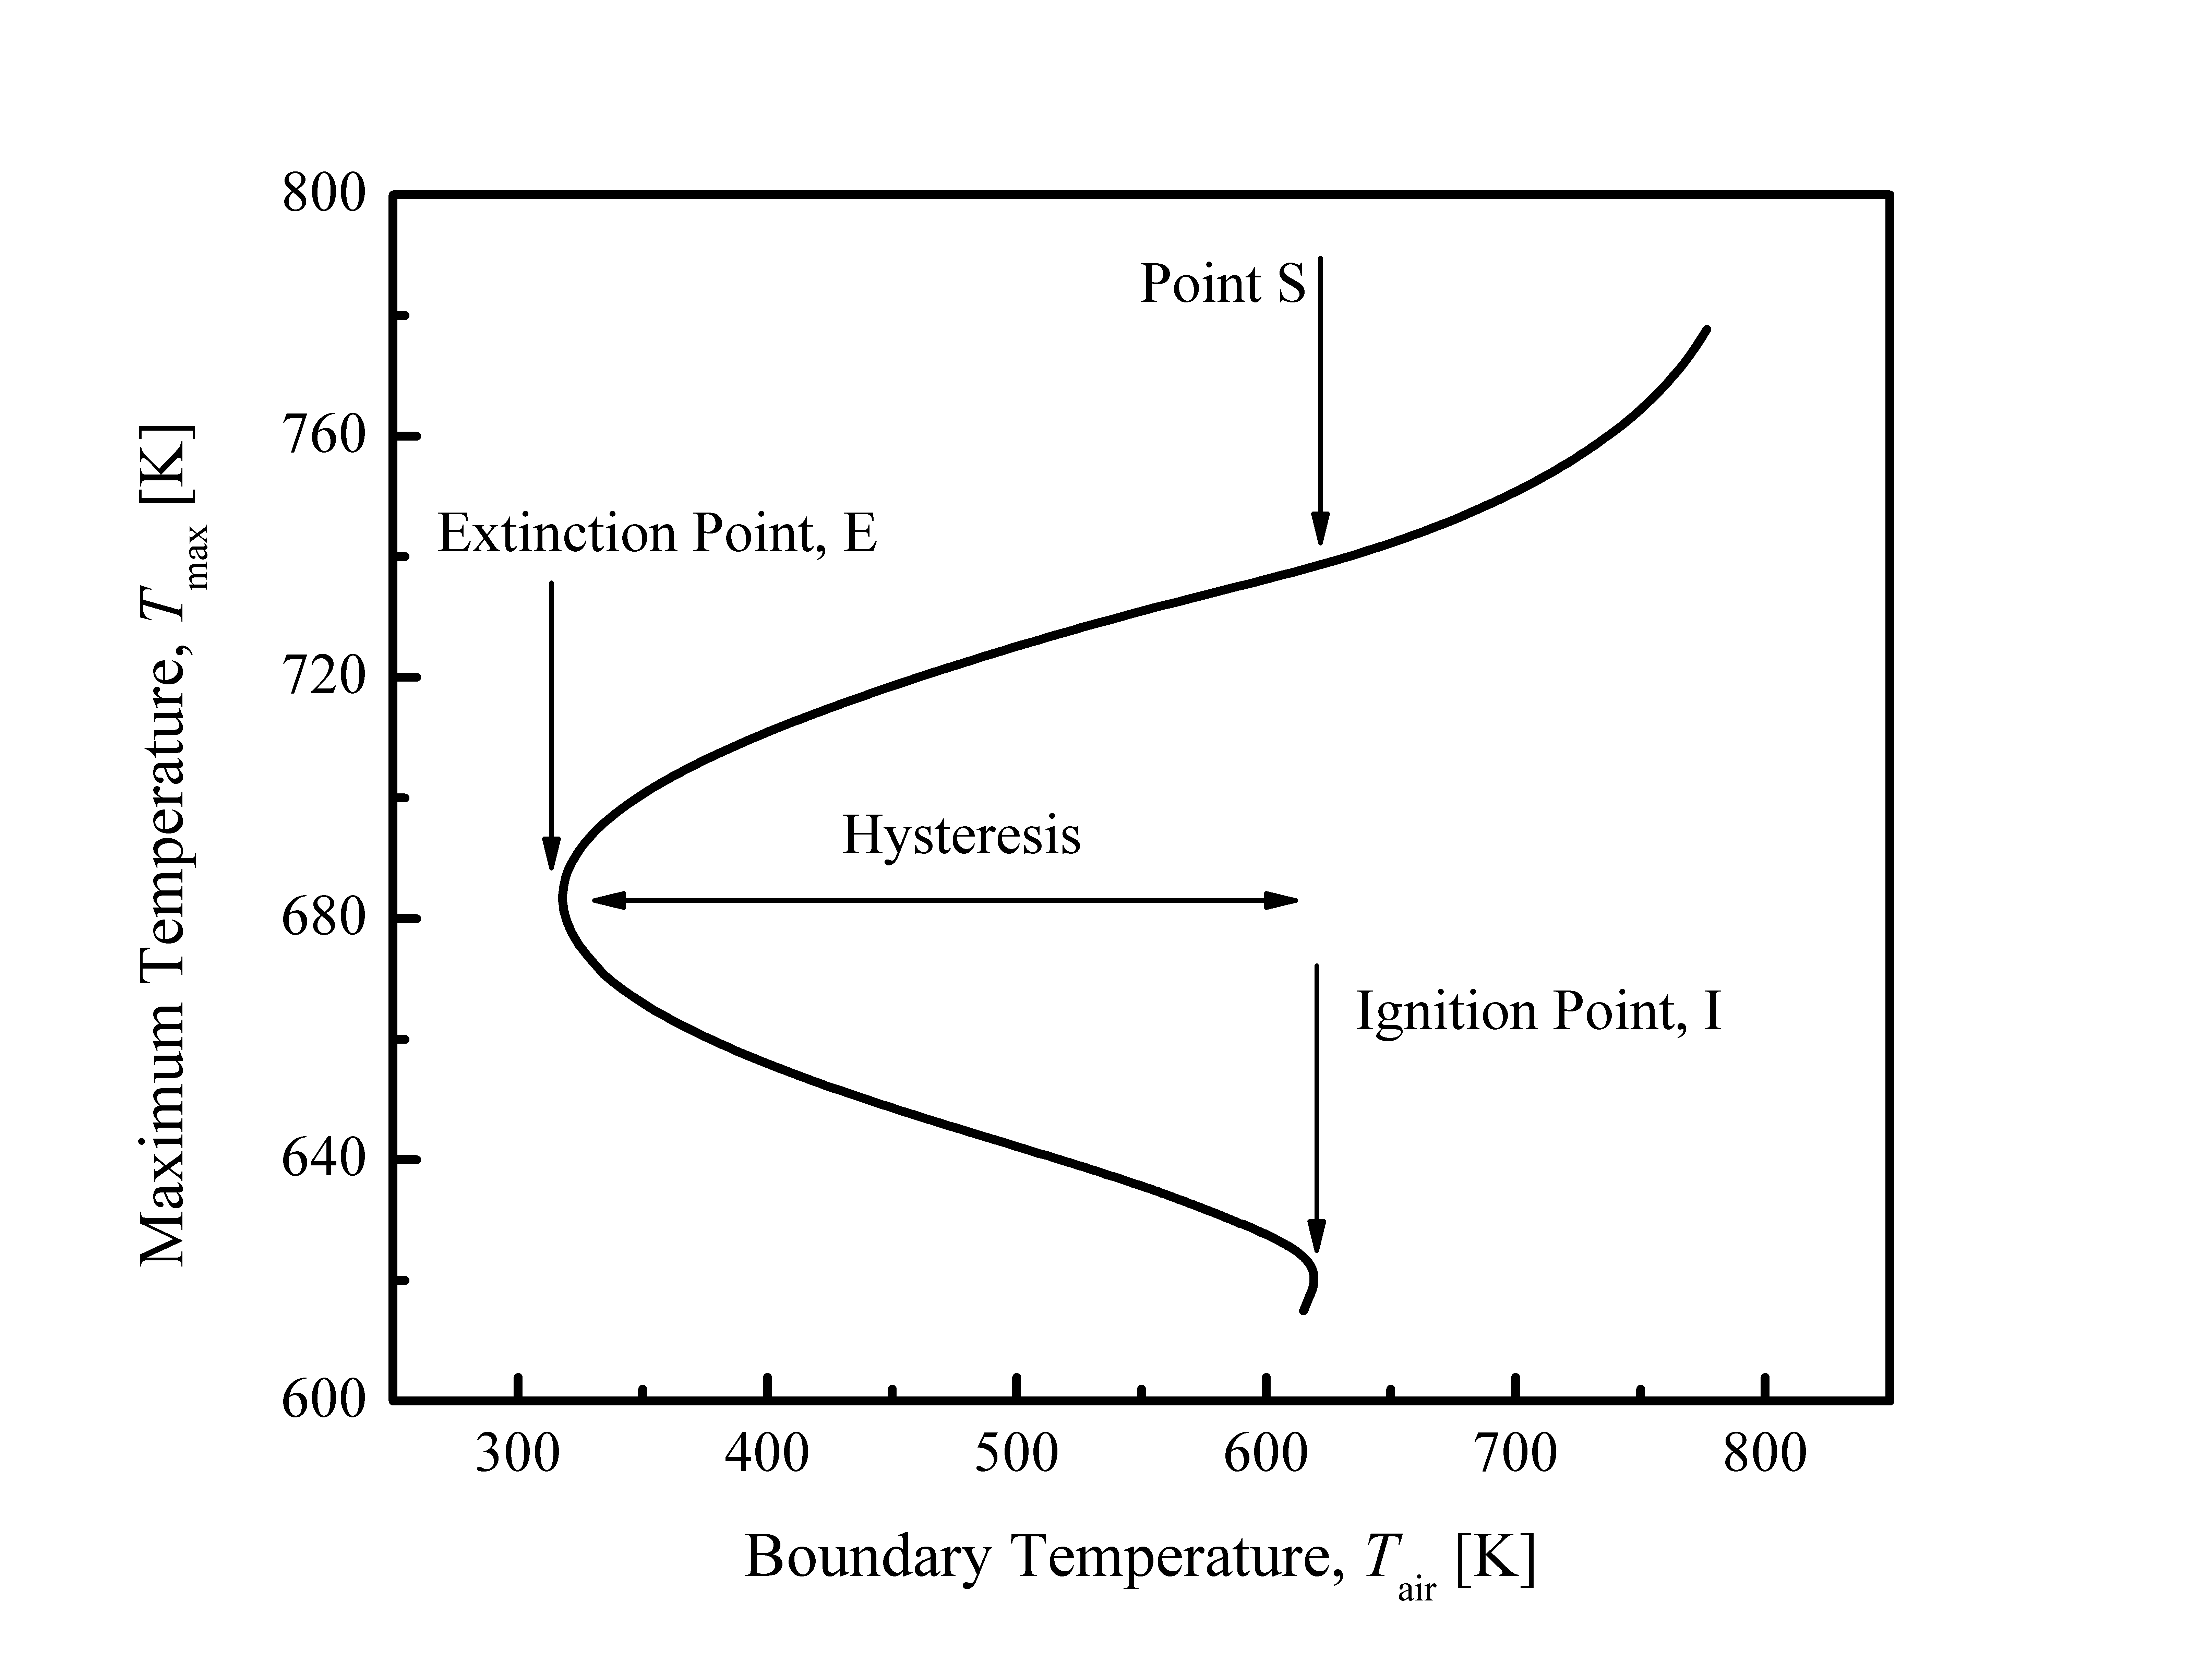
\includegraphics[trim=6.5mm 7.5mm 7mm 8mm, clip=true, width=0.5\textwidth]{S-Curve.png}
  \normalsize
  \caption{S-Curve analysis of the response of nonpremixed counterflow of 50\% DME and 50\% nitrogen versus heated air at the 2 atm and pressure-weighted strain rate of 80 /s.}
  \label{fig:S-curve}
\end{figure*}


To capture this computationally predicted hysteresis, the ignition and extinction temperatures were experimentally measured in the counterflow based on the chemiluminescence of the cool flame.  Figure~\ref{fig:UV} shows representative images of the ignition and extinction detection for the DME/air cool flame at 2 atm and pressure-weighted strain rate of 84 /s.  Ignition of the cool flame is achieved by gradually increasing the oxidizer boundary temperature.  As shown in the left column of Fig.~\ref{fig:UV}, when the oxidizer boundary temperature is slowly increased from 626 K to 637 K (A to D), the chemiluminescence from the low-temperature chemistry suddenly becomes detectable by the UV camera, indicating onset of the cool flame.  The oxidizer boundary temperature is then gradually reduced with a temperature interval of 1 K, while maintaining quasi-steadiness at each step.  The right column of Fig.~\ref{fig:UV} then shows that, while the cool flame chemiluminescence remains as the boundary temperature is decreased from 637 K to 626 K (E to H), it suddenly vanishes at 626 K, which was thus defined as the extinction temperature.

\begin{figure*}[t]
  \centering
  \scriptsize
  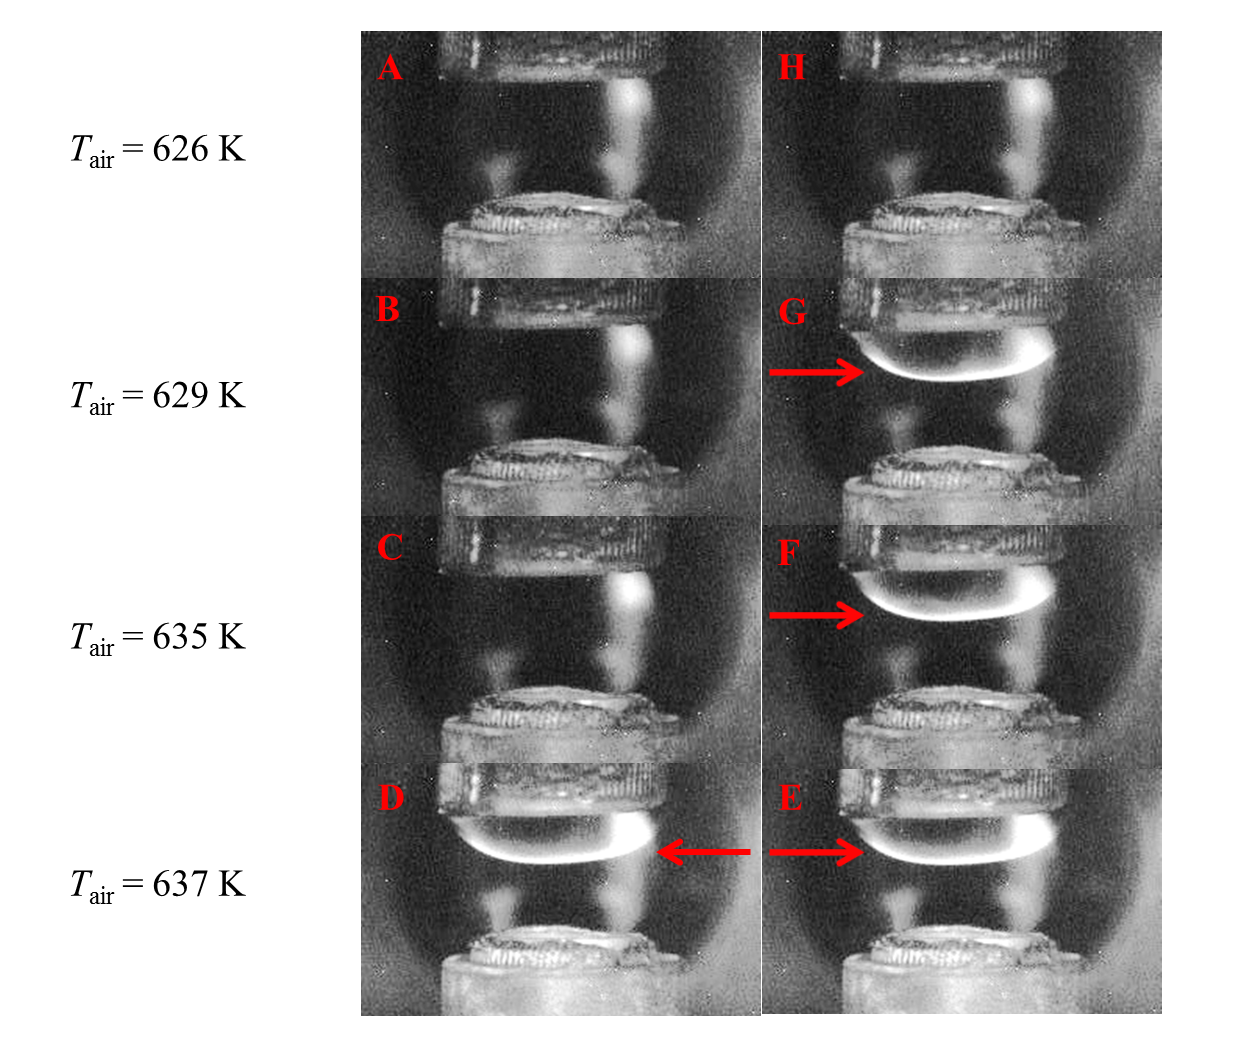
\includegraphics[trim=6.5mm 7.5mm 7mm 1mm, clip=true, width=0.5\textwidth]{UV.png}
  \normalsize
  \caption{Flame images demonstrating the hysteretic nature of ignition and extinction of cool flames with air temperature. DME cool flame at 2 atm and pressure-weighted strain rate of 84 /s; DME volume fraction in the fuel stream is 50\%, and the oxidizer stream is air.}
  \label{fig:UV}
\end{figure*}

The same procedure was followed to obtain the ignition and extinction temperatures at various strain rates for comparisons with the computationally predicted values, as shown in Fig.~\ref{fig:cmp_demo}.  Results from experiment and computation then both show that the ignition and extinction temperatures increase with increasing strain rate, due to reduced residence time.  Furthermore, the ignition temperature not only is higher than the extinction temperature at a given strain rate, it is also less sensitive to the strain rate, resulting in a less pronounced ignition-extinction hysteresis. Noting that the repeatability of the measurement is within 2 K, which is within the marker size in the figure, and the error bar represents the uncertainty of the radiation correction using different models, comparison between the experimental data should be made based on the upper or lower bound of the uncertainty bar across all the measurements.

It is also apparent from Fig.~\ref{fig:cmp_demo} that while the experimental and computational results separately exhibit the anticipated physics, namely the extinction temperature is lower than the ignition temperature, and they both increase with increasing strain rate, the quantitative comparison between them is overall poor, both in magnitude as well as the strain-rate sensitivity. We shall defer the detailed analysis of these discrepancies to Sec.~\ref{sec:uncertainty}. 

\begin{figure*}[t]
  \centering
  \scriptsize
  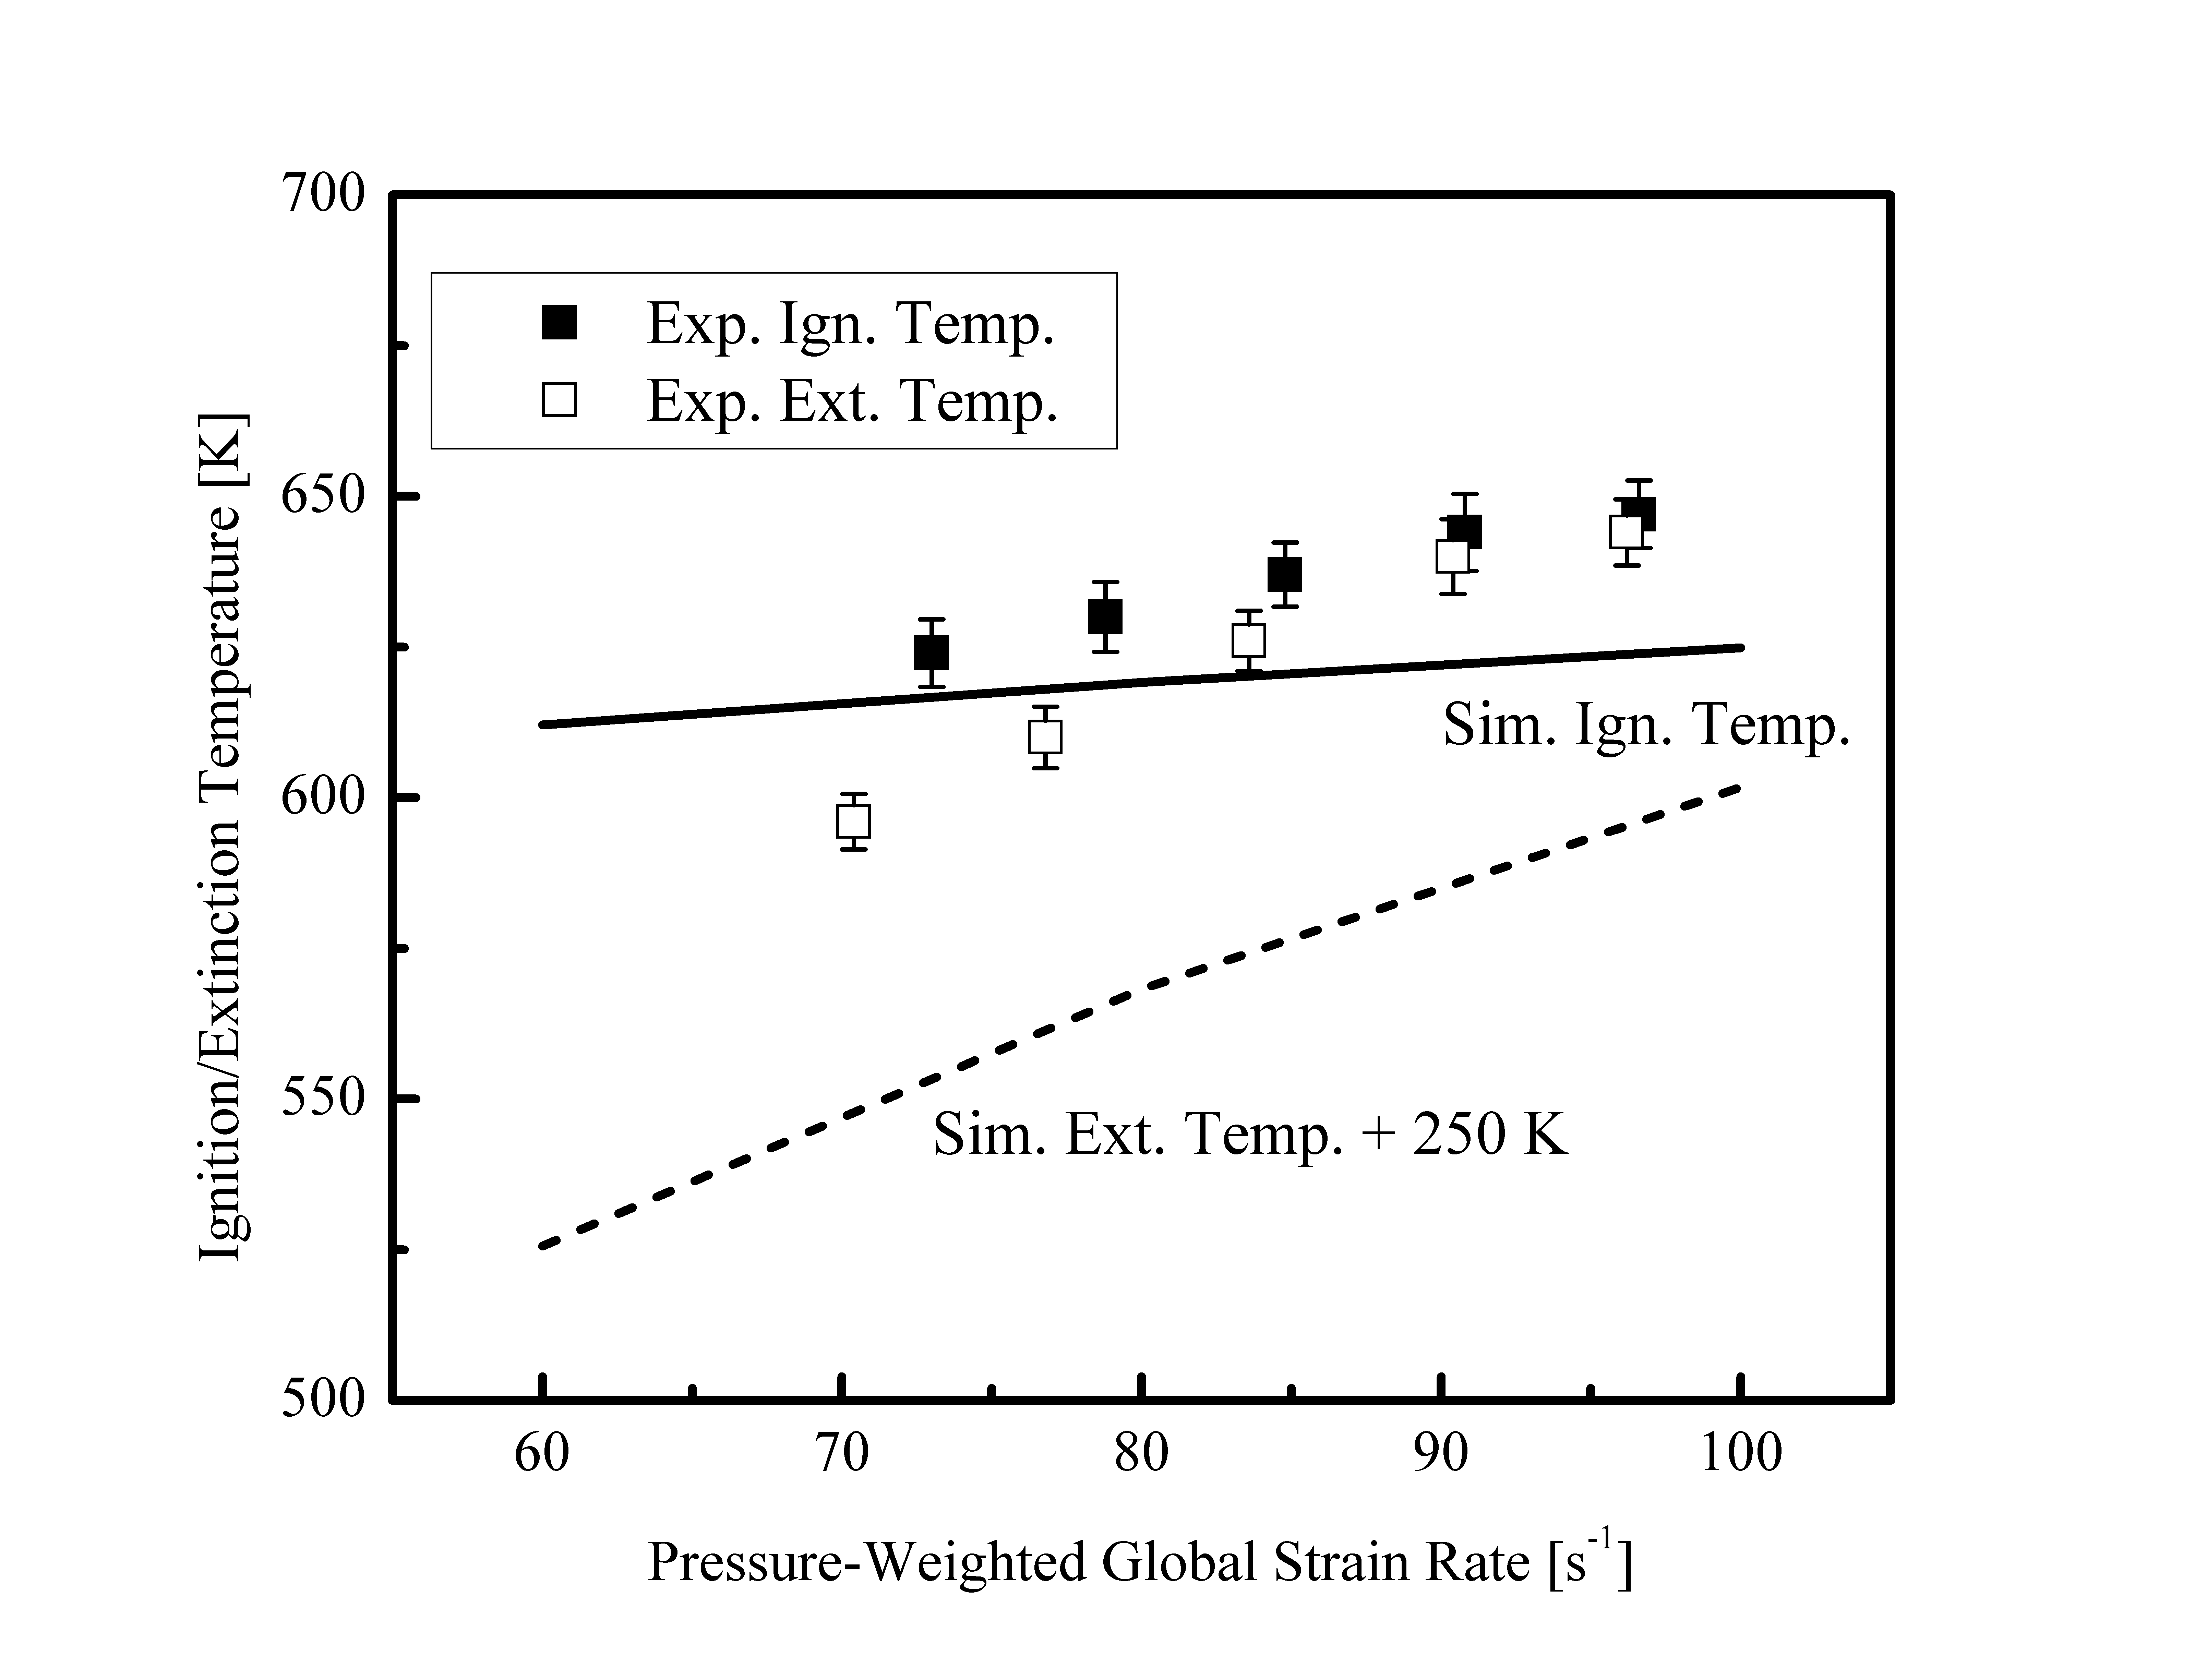
\includegraphics[trim=6.5mm 7.5mm 7mm 8mm, clip=true, width=0.5\textwidth]{cmp_demo.png}
  \normalsize
  \caption{Experimental and computed ignition and extinction temperatures at 2 atm and various strain rates.  The computed extinction temperature is shifted up by 250 K for better illustration.  DME volume fraction in the fuel stream is 50\%, and the oxidizer stream is air.}
  \label{fig:cmp_demo}
\end{figure*}

\subsection{Analysis of thermal and chemical structures}\label{sec:structure}

In order to elucidate the dominant chemical pathways and evolution of the ignition and extinction processes, the three characteristic points on the S-curve of Fig.~\ref{fig:S-curve}, which respectively represent the states prior to ignition (point I), steady burning (point S), and prior to extinction (point E), were chosen for structural analysis.

As shown in Fig.~\ref{fig:HRR}, the heat release just prior to the initiation of the cool flame is negligible, and the maximum temperature in the flow field is set by the oxidizer boundary.  For both steady flames at points S and E, there are reaction kernels delineated by the heat release profiles.  Based on the full width at half maximum of the heat release profile, a typical cool flame thickness is about 0.05 cm for the present conditions.  At point E, the heat release rate of the cool flame is higher than that at point S, for low-temperature chemistry is favored at relatively lower temperatures.  However, the steep gradient of the heat release profile indicates that heat loss due to strain at point E is more pronounced compared to point S.  As the boundary temperature further decreases, such heat loss increases, and chemical reactions cannot keep up with heat loss from the reaction zone, leading to extinction due to the limited residence time in the strained flow.

\begin{figure*}[t]
  \centering
  \scriptsize
  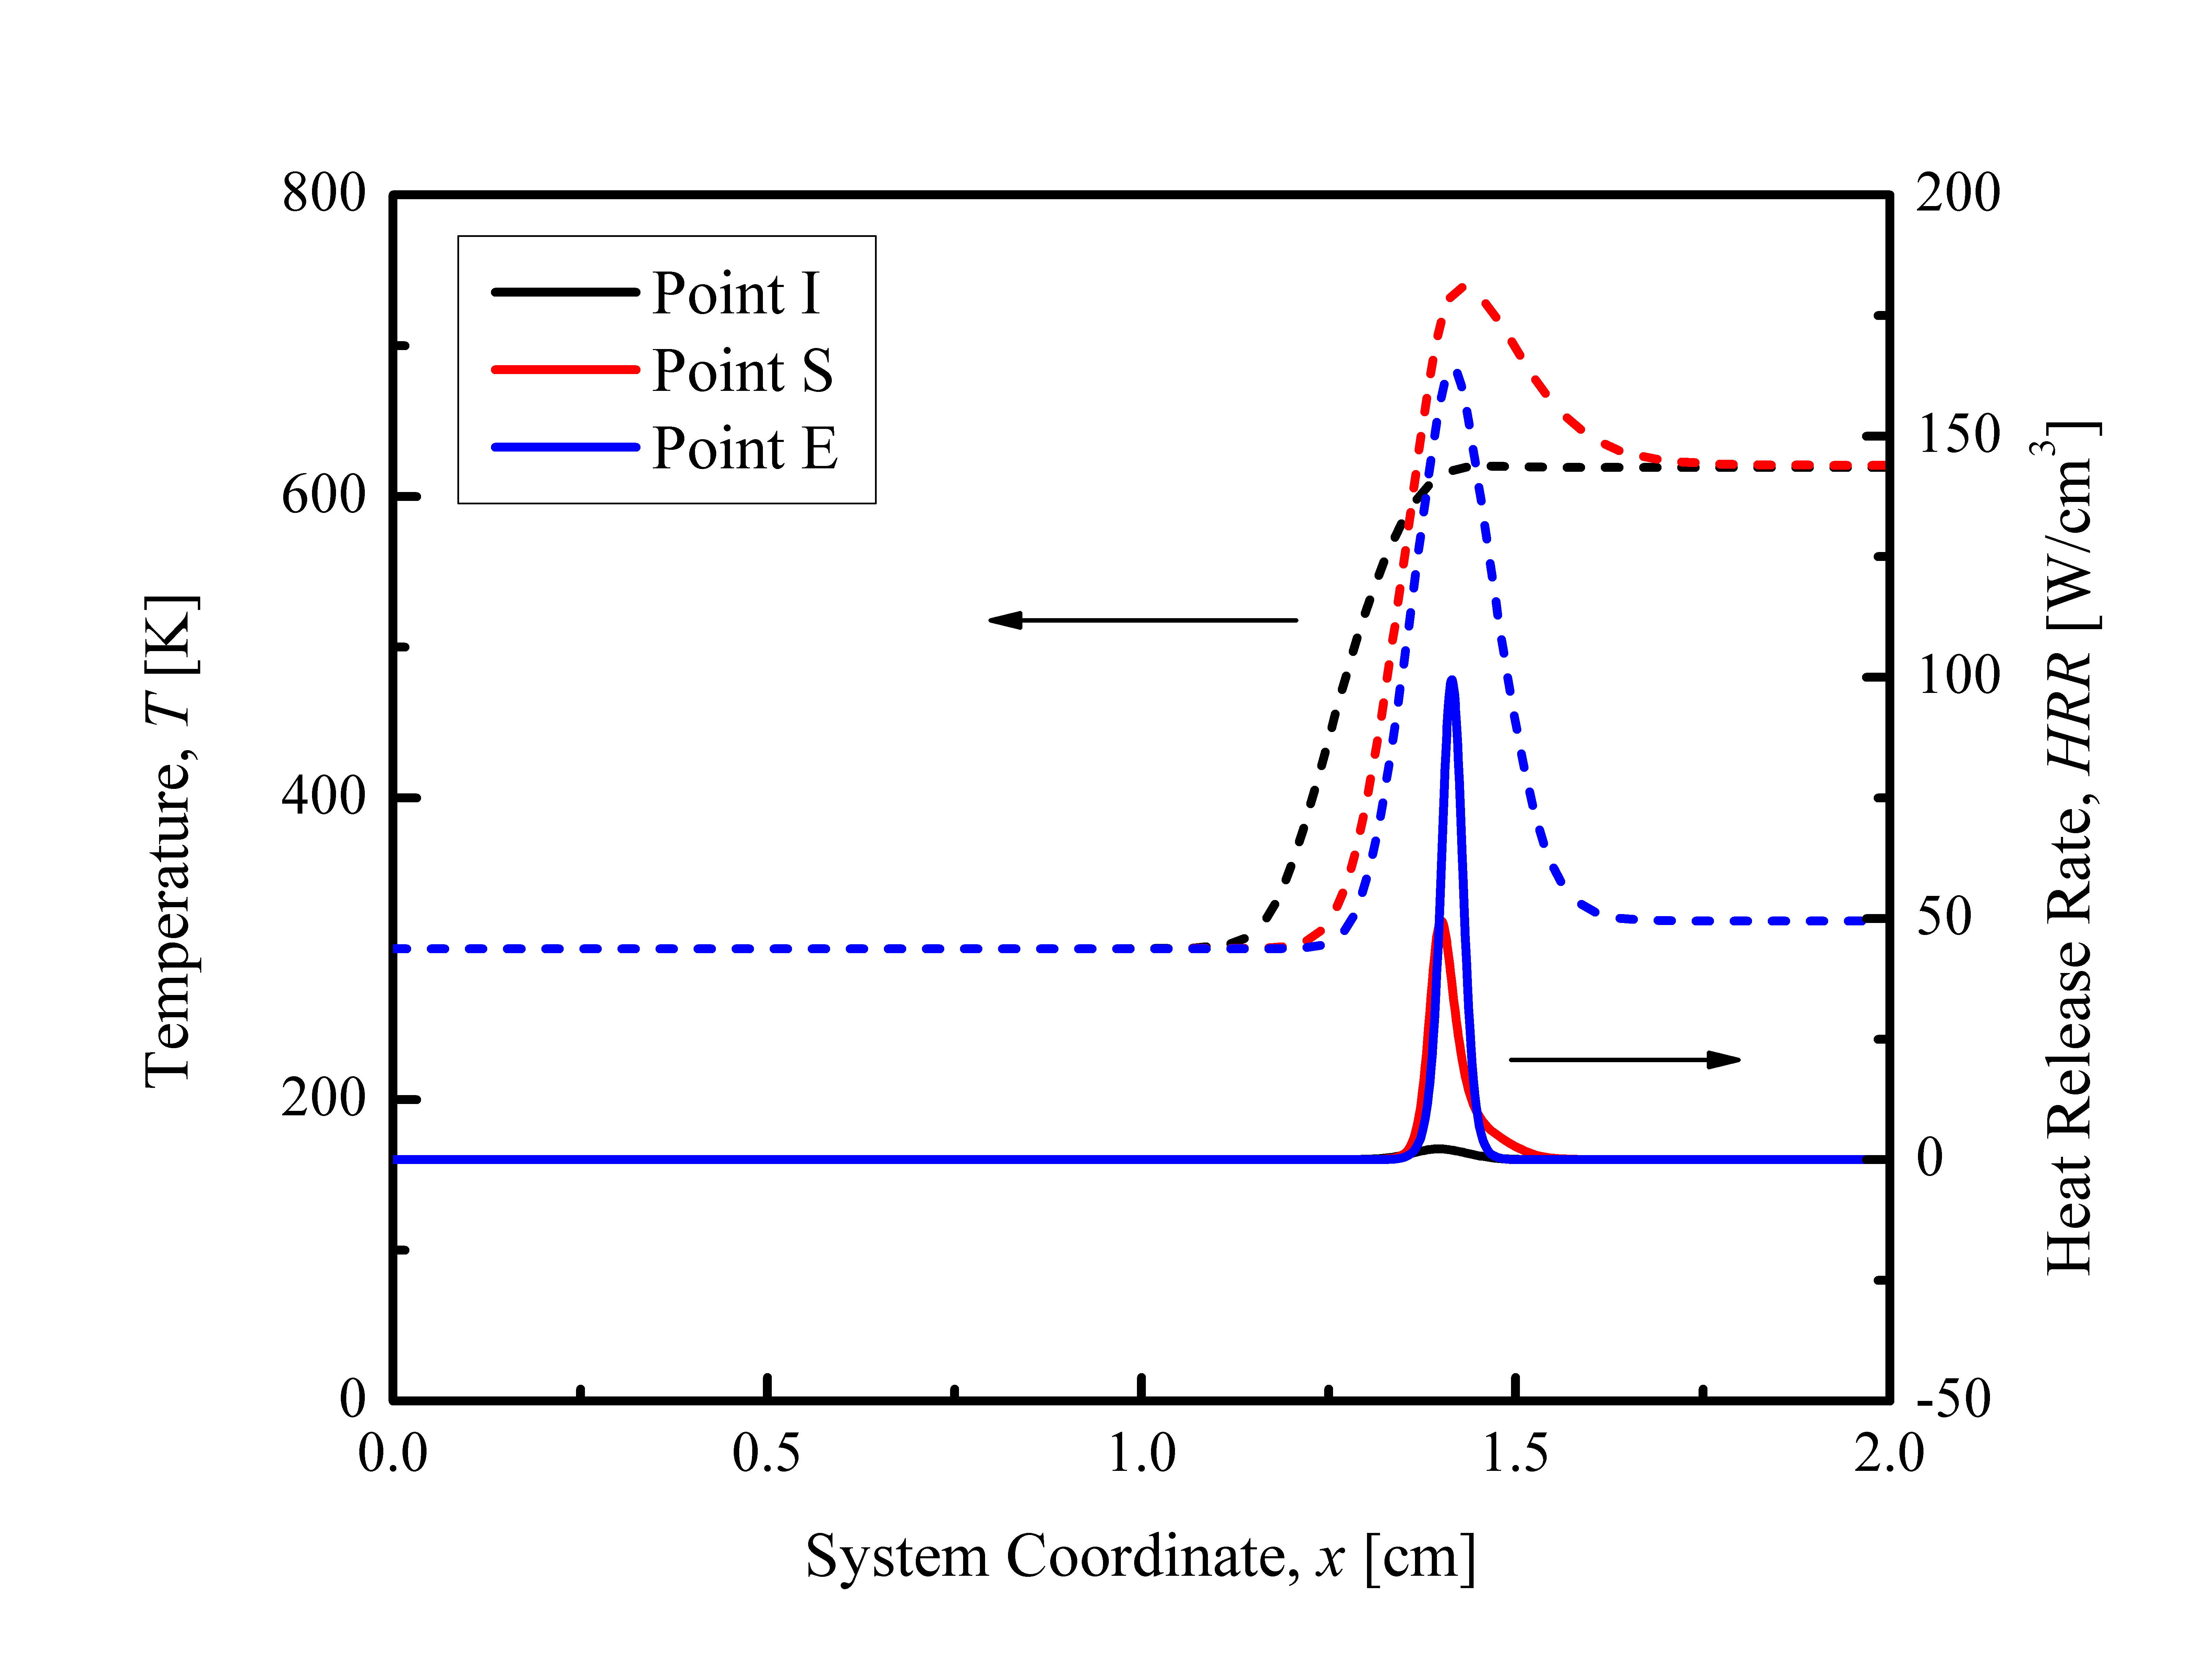
\includegraphics[trim=6.5mm 7.5mm 7mm 8mm, clip=true, width=0.5\textwidth]{HRR.png}
  \normalsize
  \caption{Thermal structures in the computed flow field at three representative points on the S-curve shown in Fig.~\ref{fig:S-curve}.  \textcolor{Rev1}{The solid lines refer to heat release rate, while the dashed lines refer to temperature.}  Fuel stream boundary conditions are specified at $x=0$ in the computation.}
  \label{fig:HRR}
\end{figure*}

\begin{figure*}[t]
  \centering
  \scriptsize
  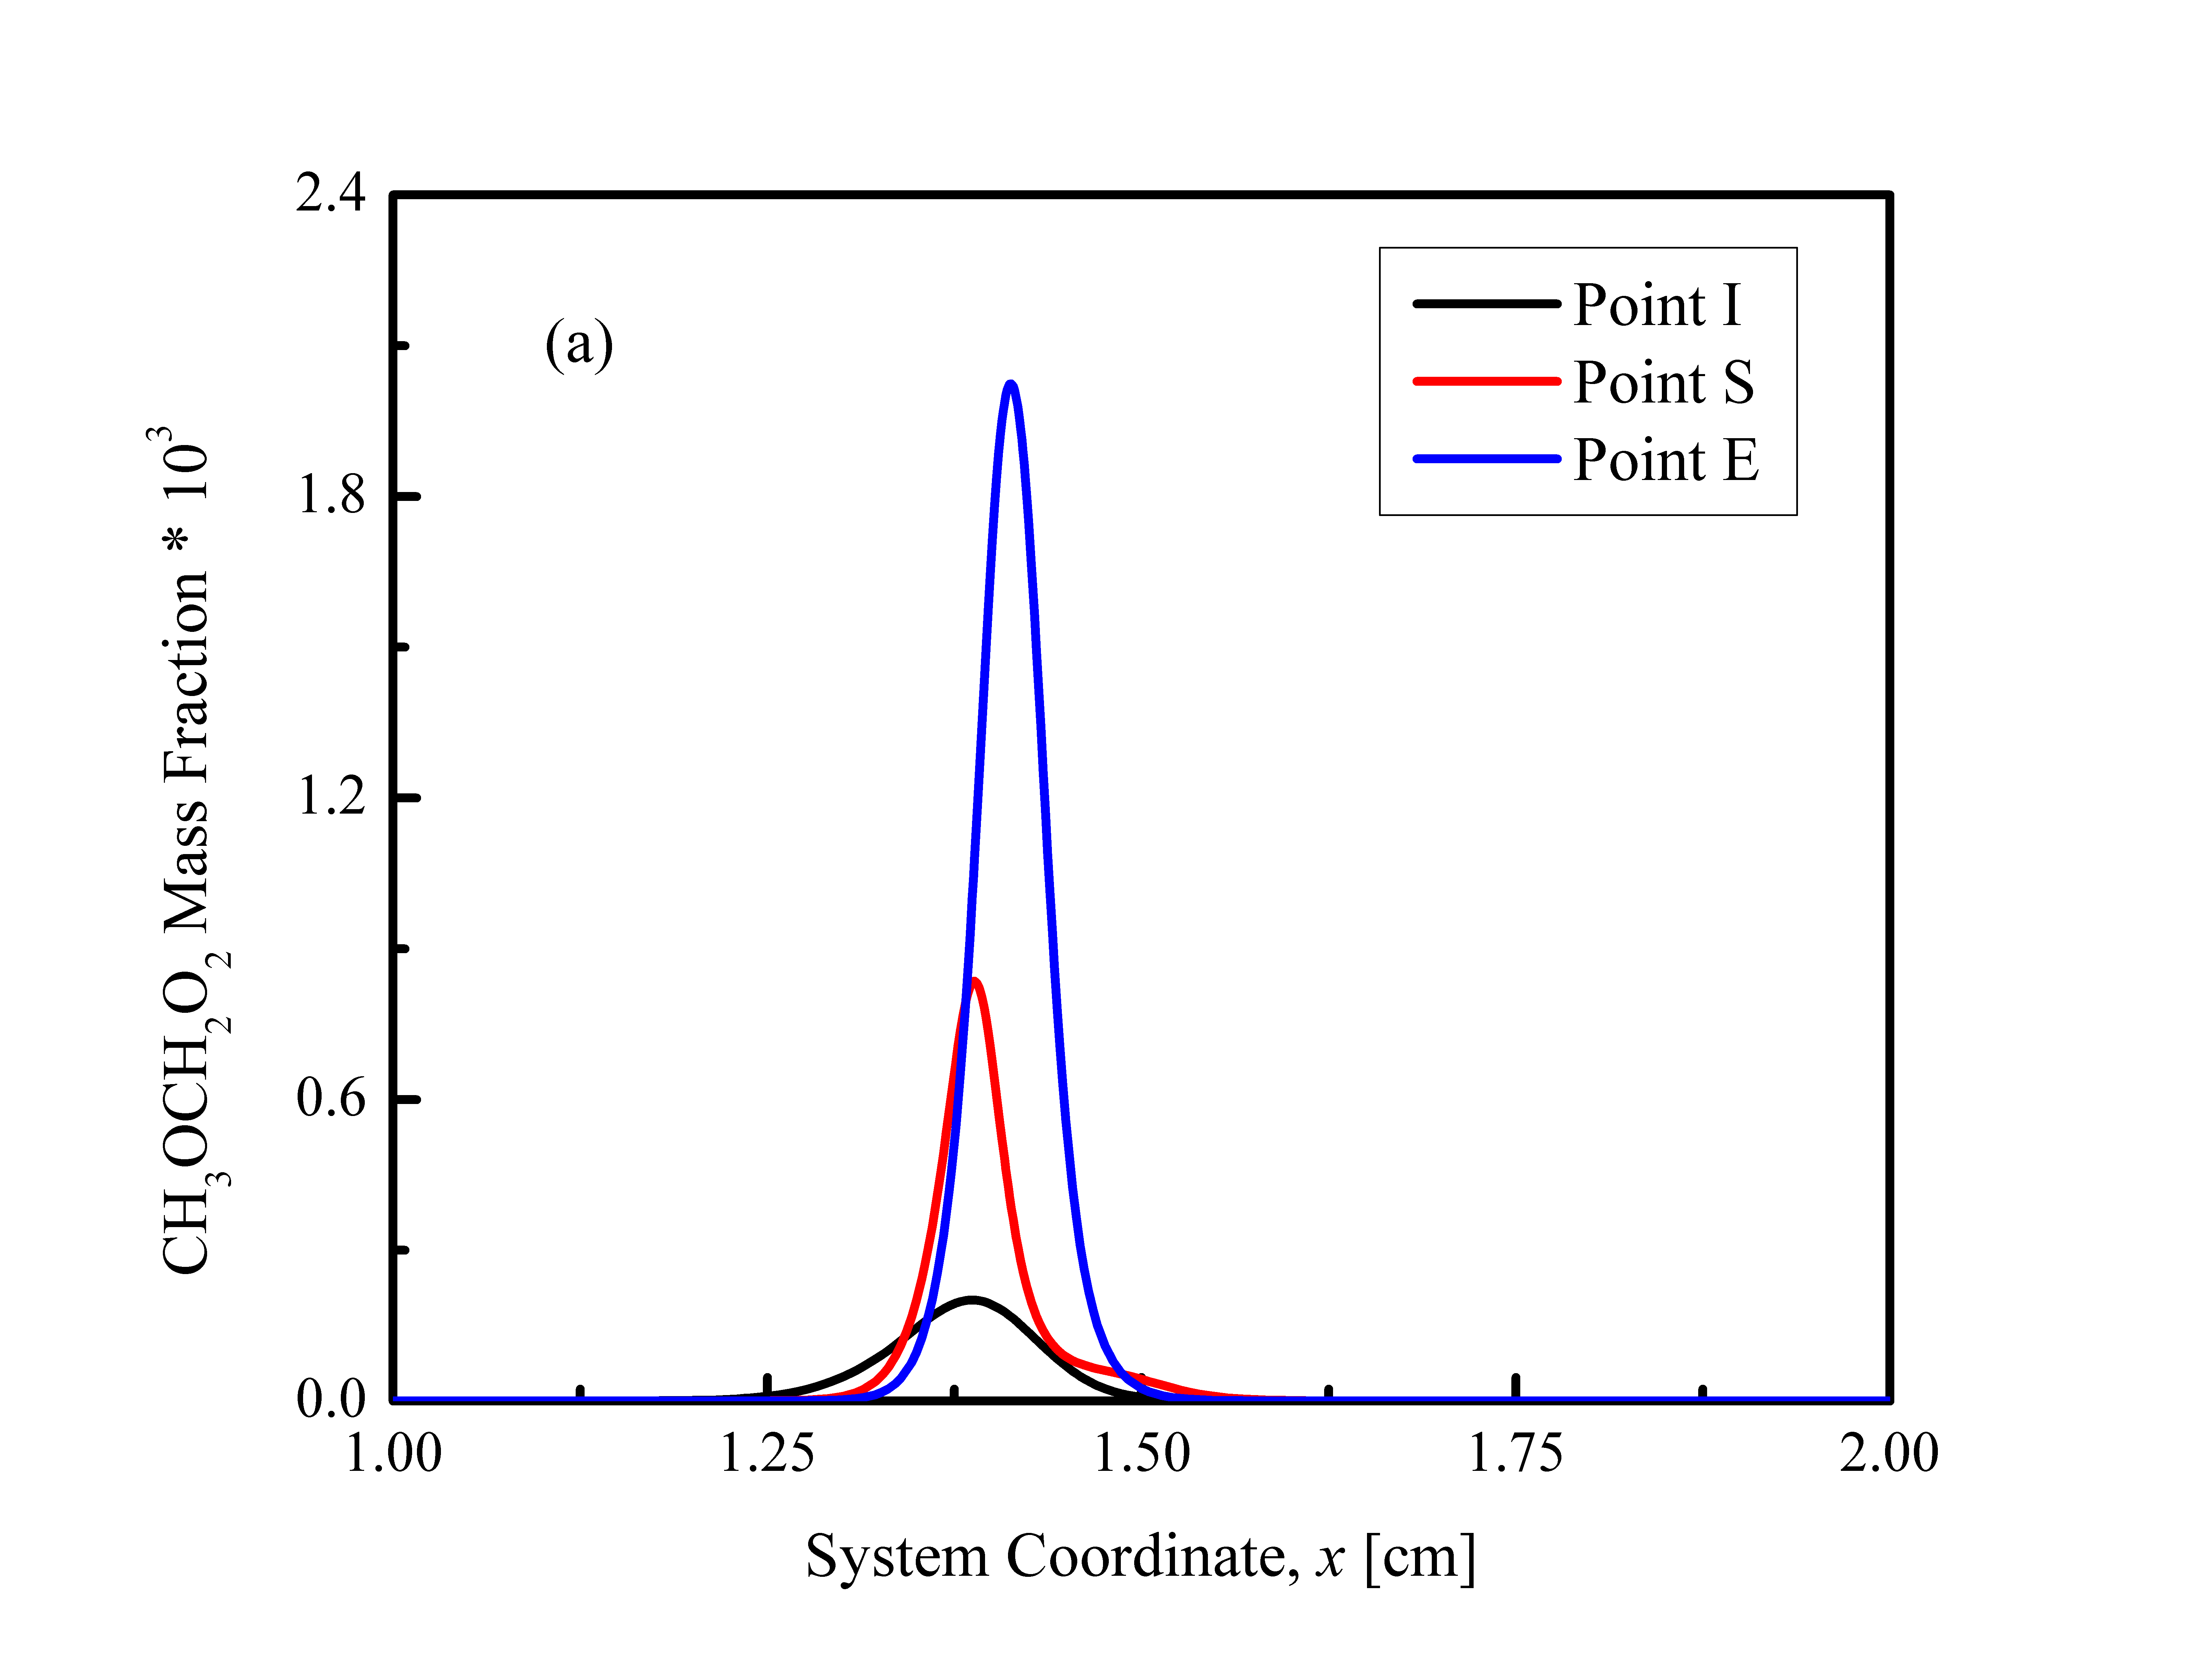
\includegraphics[trim=6.5mm 7.5mm 7mm 8mm, clip=true, width=0.5\textwidth]{sp_a.png}
  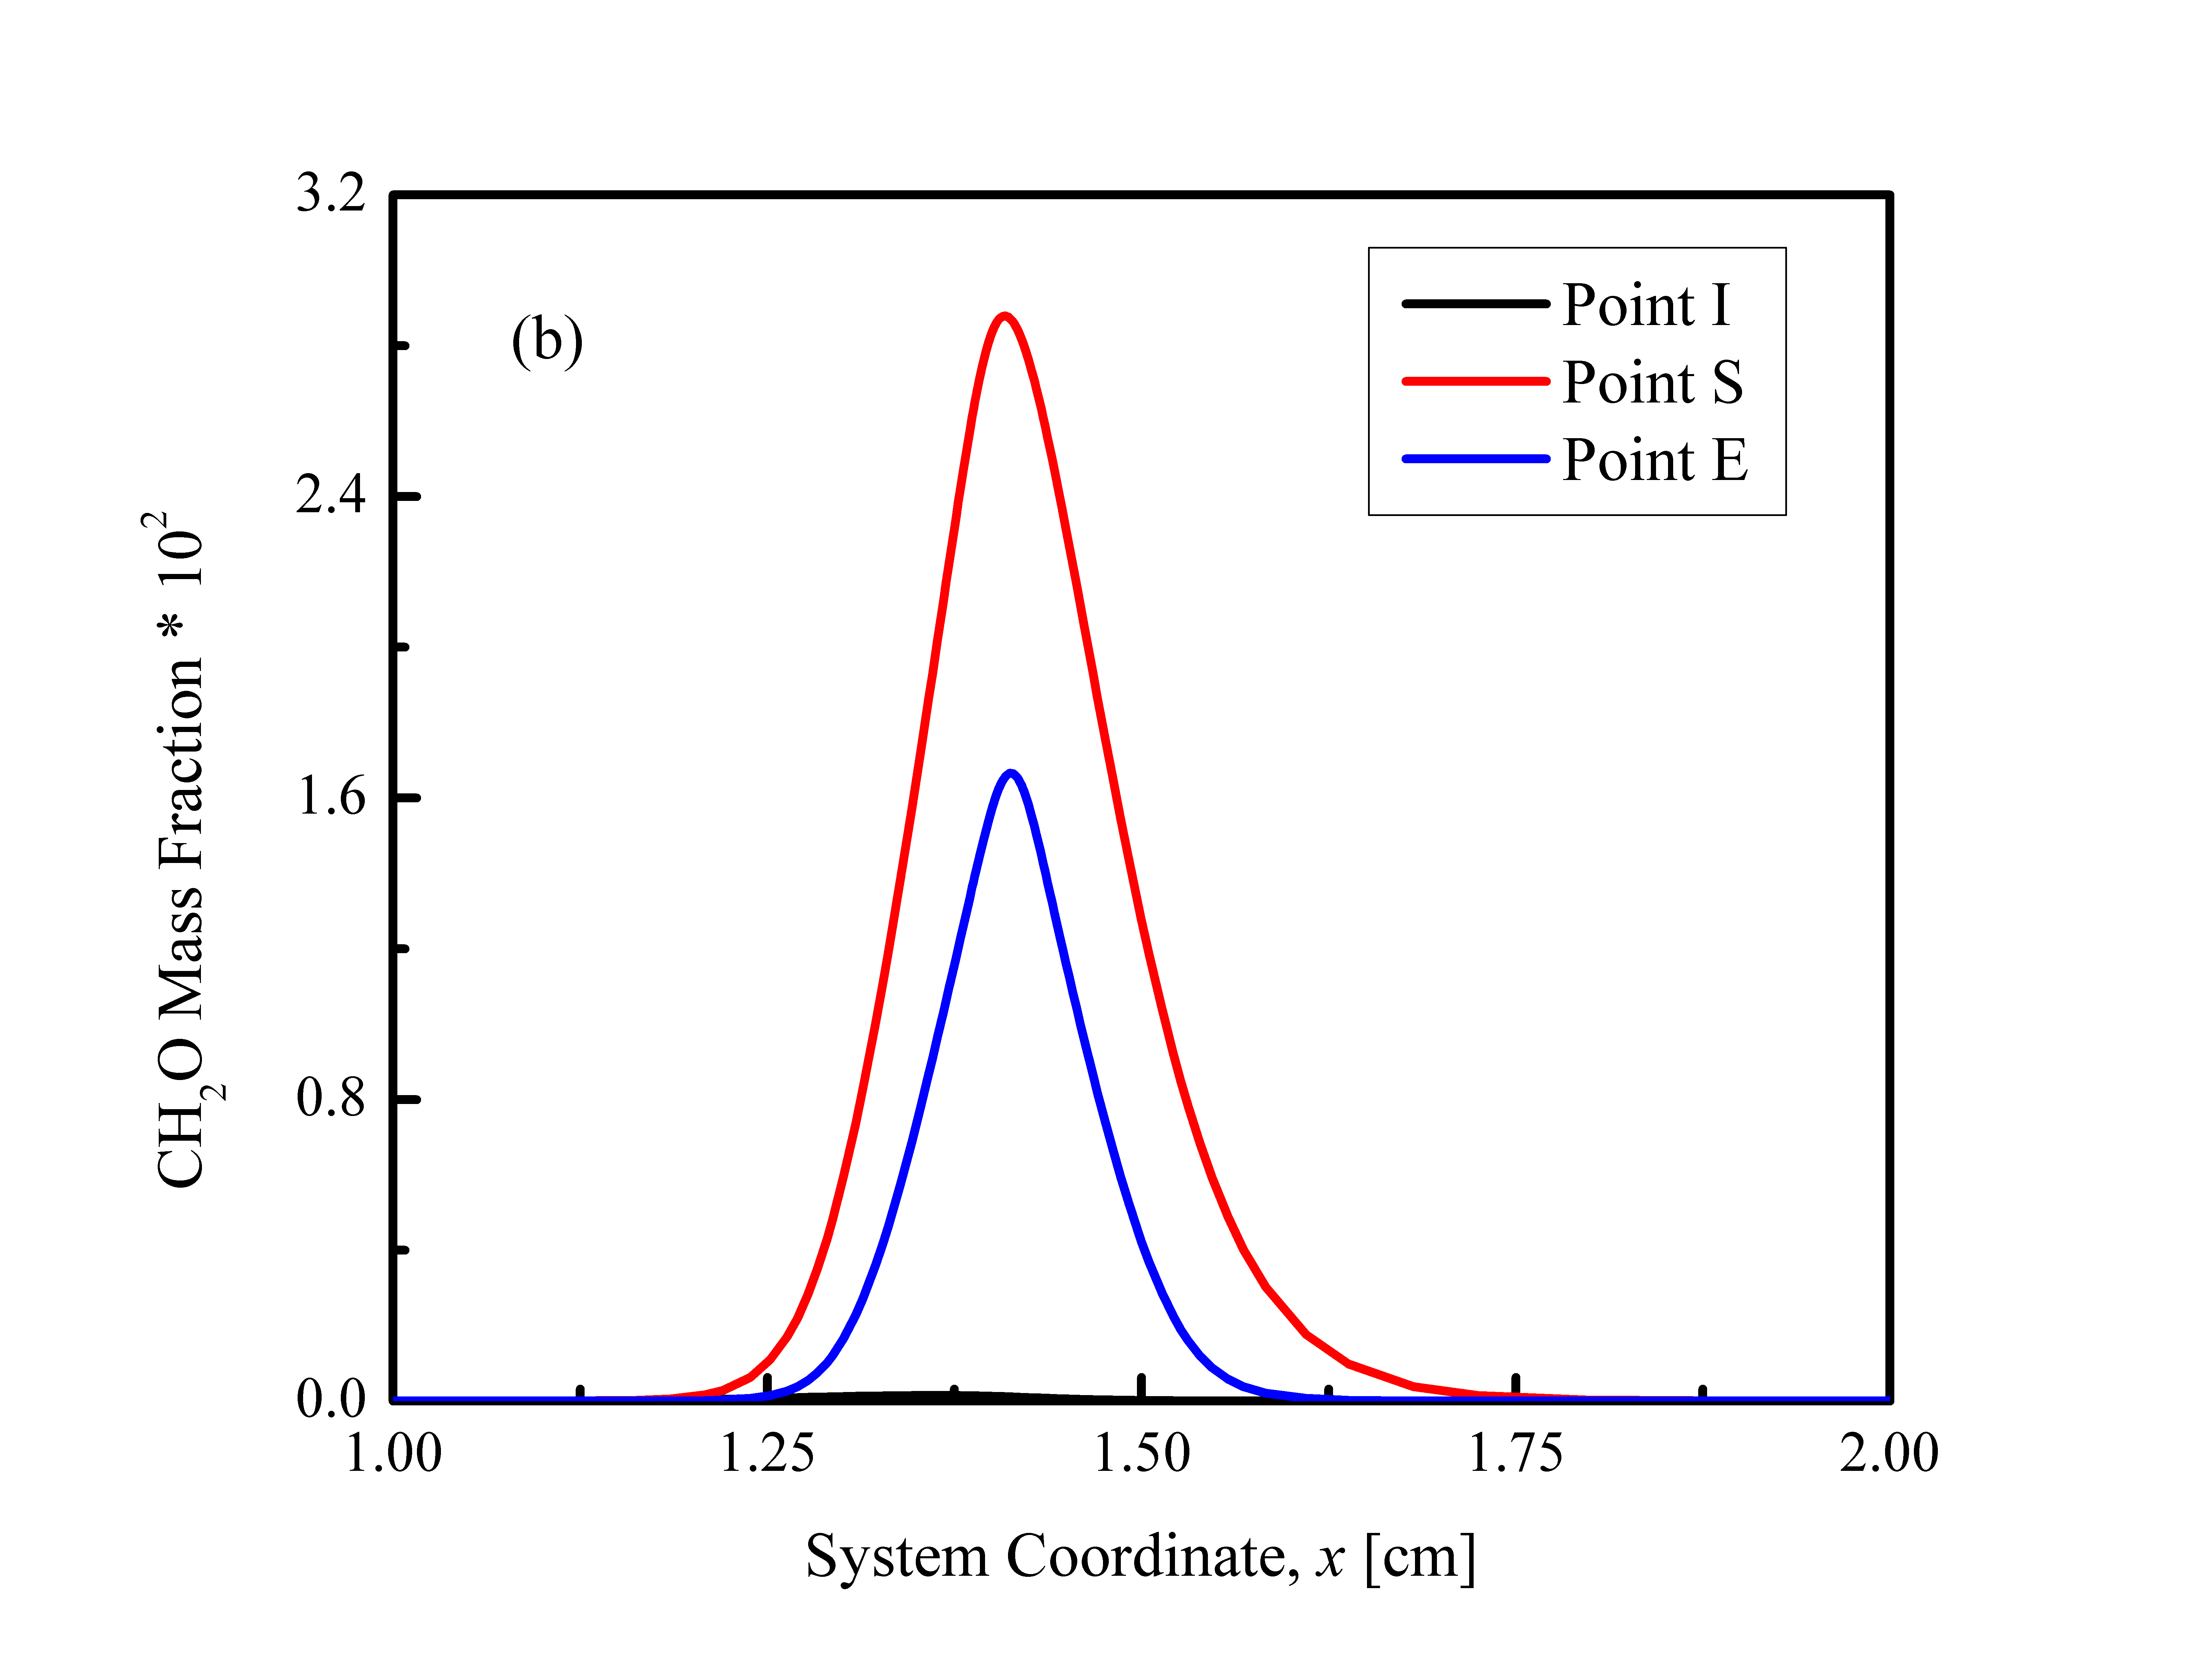
\includegraphics[trim=6.5mm 7.5mm 7mm 8mm, clip=true, width=0.5\textwidth]{sp_b.png}
  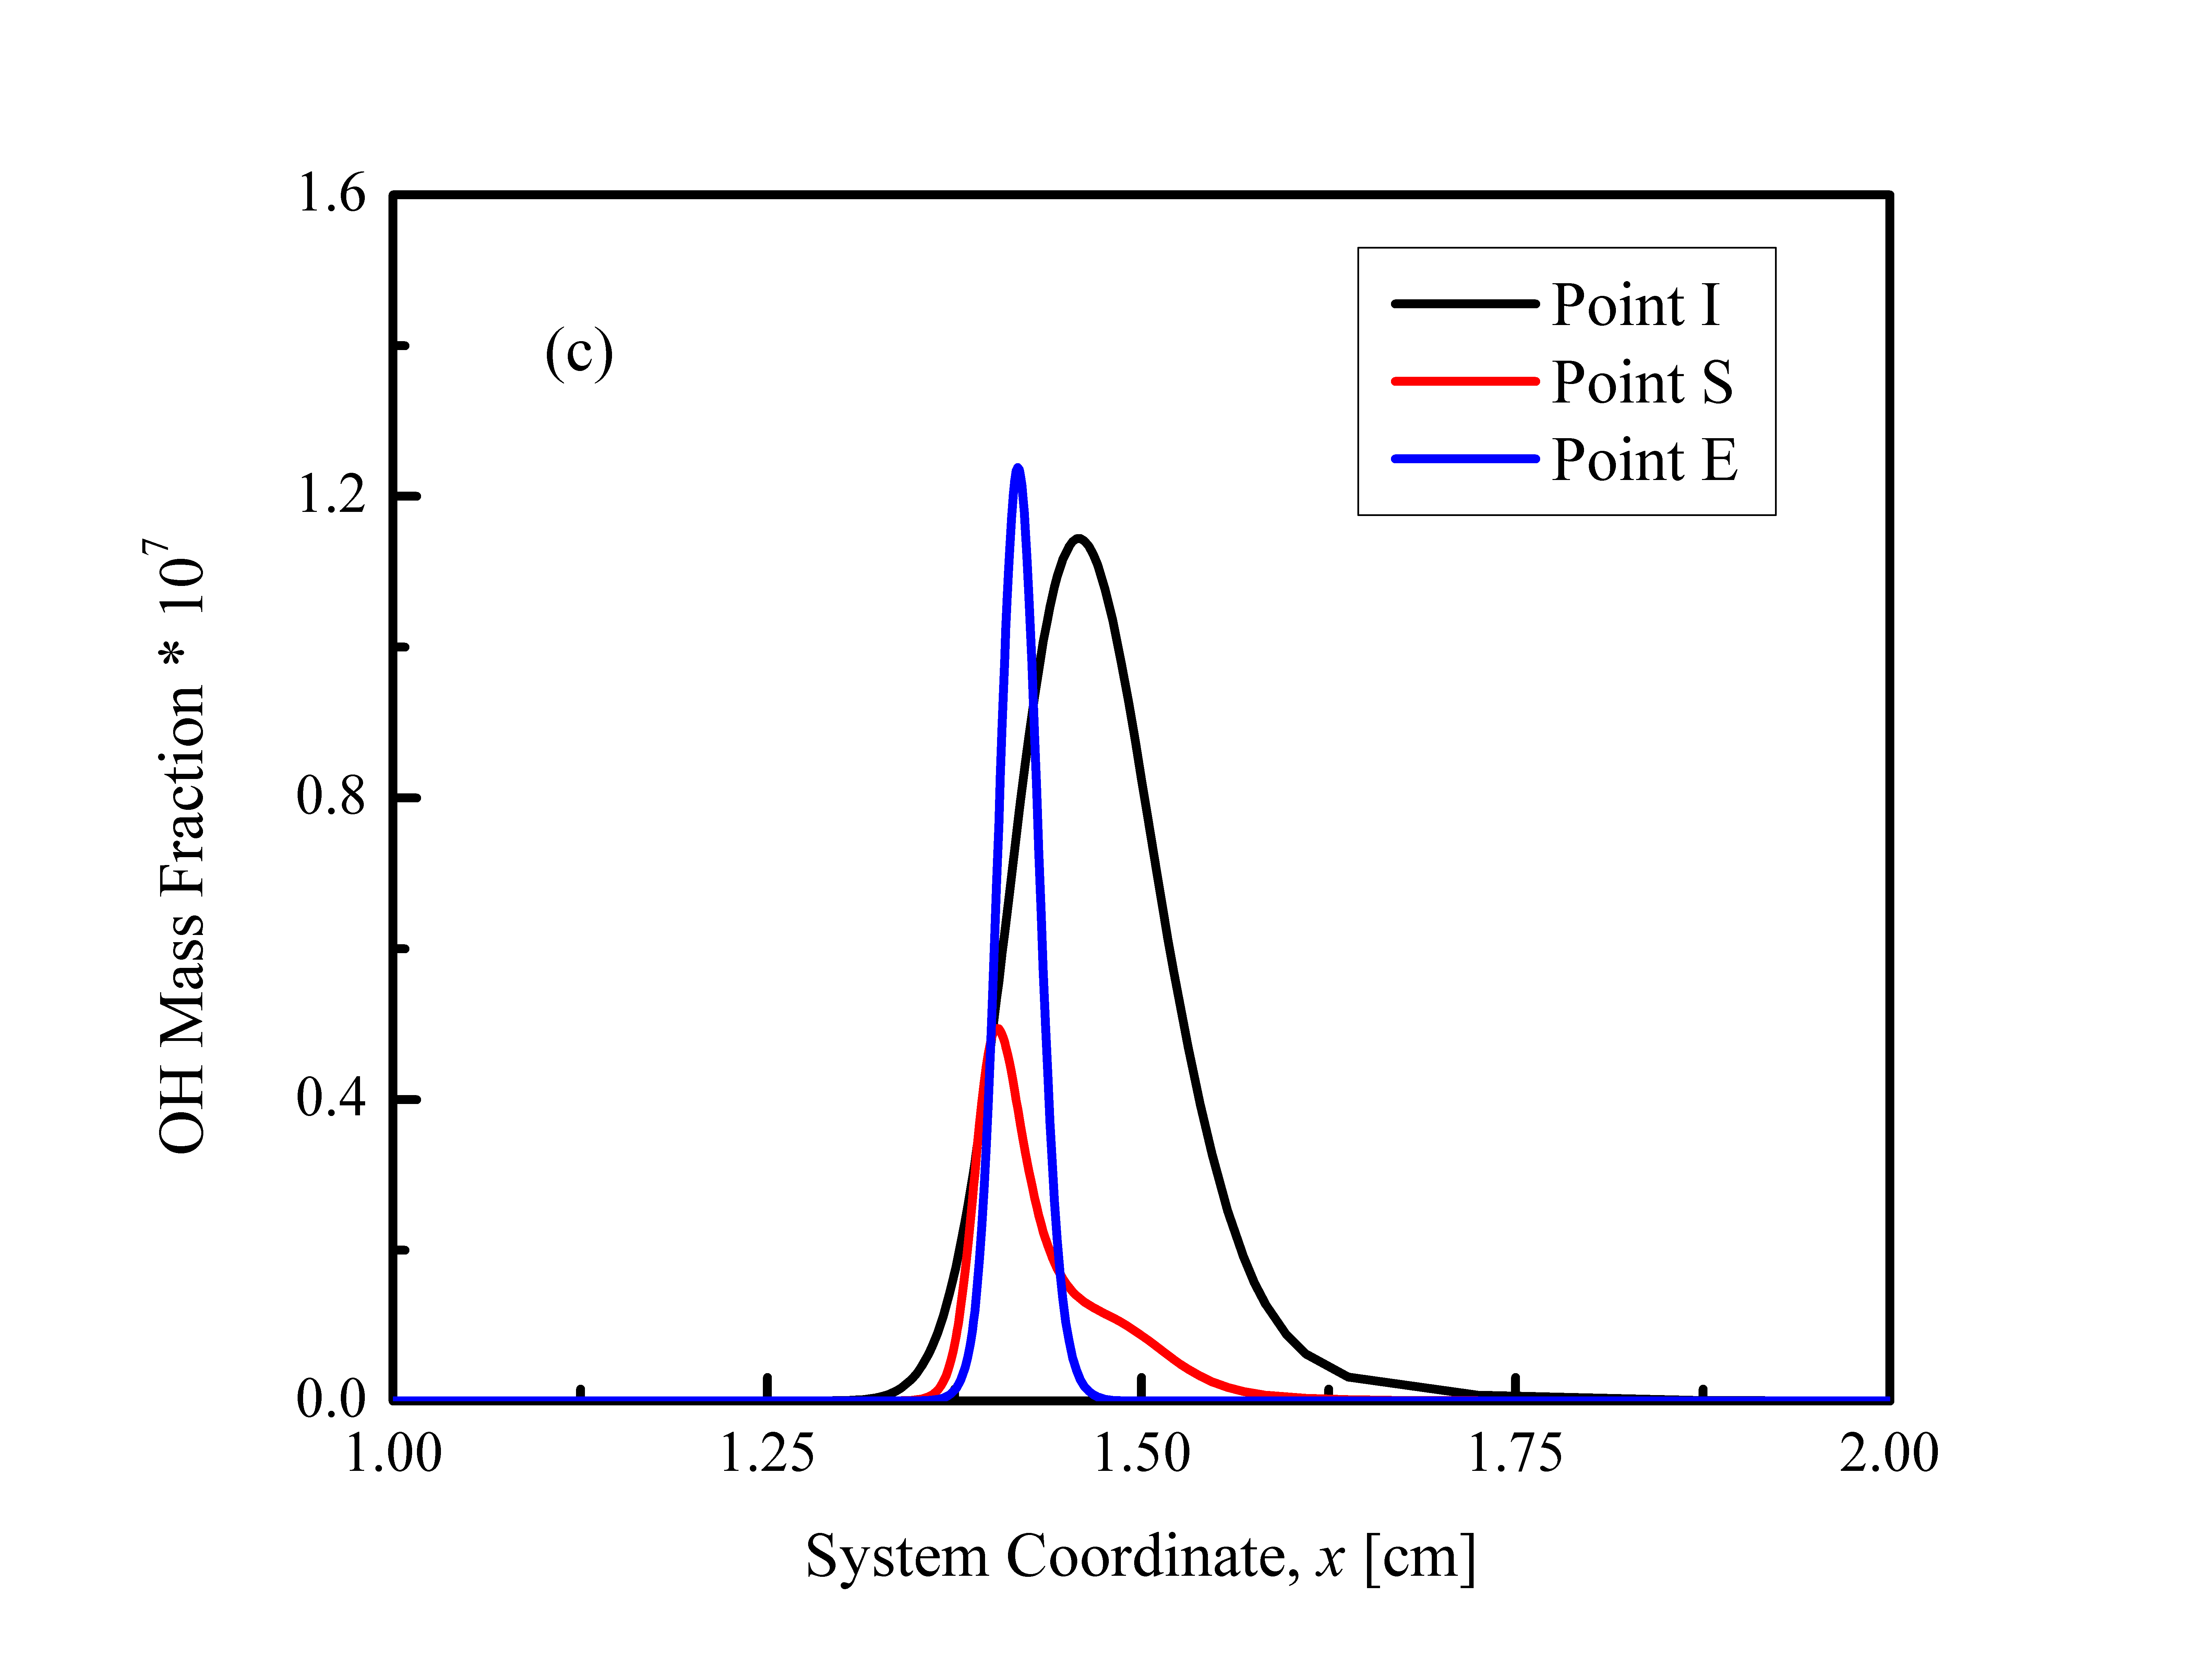
\includegraphics[trim=6.5mm 7.5mm 7mm 8mm, clip=true, width=0.5\textwidth]{sp_c.png}
  \normalsize
  \caption{(a) Methoxymethylperoxy radical, (b) formaldehyde, and (c) hydroxyl radical profiles in the computed flow field at three representative points on the S-curve shown in Fig.~\ref{fig:S-curve}.  Fuel stream boundary conditions are specified at $x=0$ in the computation.}
  \label{fig:species}
\end{figure*}

The profiles of three representative species, namely methoxymethylperoxy (CH$_3$OCH$_2$O$_2$), formaldehyde (CH$_2$O), and hydroxyl (OH), were then investigated to elucidate the chemical structures at these three points, I, S, and E, as shown in Fig.~\ref{fig:species}.  The methoxymethylperoxy radical was chosen because it is a representative species for the low-temperature chemistry~\cite{deng15,deng15b}.  Comparing the species profiles of the three states, it is seen that the CH$_3$OCH$_2$O$_2$ mass fraction increases upon flame initiation, and similar to the heat release rate profile, its peak increases as extinction is approached.  Moreover, the profile broadens for low-temperature chemistry is favored at reduced oxidizer boundary temperature.  Formaldehyde was selected because it is a major “product” of the cool flame, with its intensity manifested through its chemiluminescence~\cite{zhao16}.  It is then seen that: negligible CH$_2$O is formed prior to ignition; significant amount is formed in the steady flame; and the concentration and hence the intensity of chemiluminescence is reduced as extinction is approached. Finally, the hydroxyl radical was chosen because it represents high-temperature flame chemistry and is also an important radical formed during the chain branching reactions of the low-temperature chemistry.  It is then noted that the peak mass fraction of OH is several orders of magnitude smaller than those in a typical hot flame\textcolor{Rev1}{~\cite{deng15b}}.  The ignition of cool flame is initiated with a peak formation of OH, which subsequently decreases upon ignition.  With subsequent heat release from the cool flame, a second peak of OH mass fraction emerges on the oxidizer side of the cool flame peak, which is responsible for the initiation of the hot flame at higher boundary temperatures~\cite{law12}.

Finally, sensitivity analysis was conducted to elucidate the evolution of the dominant chemical pathways during the ignition and extinction processes.  The maximum temperature was chosen as the target for sensitivity analysis, and the ratio of the relative change of the maximum temperature to that of the Arrhenius factor of each reaction being perturbed was defined as the sensitivity coefficient.  The sensitivity coefficients of all the reactions considered in the chemical mechanism were normalized by the maximum value such that the normalized sensitivity coefficient is bounded by -1 and 1 to allow for comparisons between the cases.

The normalized sensitivity coefficients ranked by their absolute values for states I, S, and E in Fig.~\ref{fig:S-curve} are shown in Fig.~\ref{fig:SA}.  At all three states, low-temperature chemistry is dominant, with the absence of the typical high-temperature chain branching reactions such as $\rm{H} + \rm{O}_2 \Longleftrightarrow \rm{OH} + \rm{O}$.  Similar to the ignition analysis in Deng \emph{et al.}~\cite{deng14}, the isomerization reaction $\rm{CH}_3\rm{OCH}_2\rm{O}_2 \Longleftrightarrow \rm{CH}_2\rm{OCH}_2\rm{O}_2\rm{H}$ and the oxygen addition reaction $\rm{CH}_2\rm{OCH}_2\rm{O}_2\rm{H} + \rm{O}_2 \Longleftrightarrow \rm{O}_2\rm{CH}_2\rm{OCH}_2\rm{O}_2\rm{H}$ promote ignition, while the reaction $\rm{CH}_2\rm{OCH}_2\rm{O}_2\rm{H} \Longleftrightarrow \rm{OH} + 2\rm{CH}_2\rm{O}$ retards it.  \textcolor{Rev1}{The species profiles demonstrated in Fig.~\ref{fig:species} also support such findings, for the mass fraction of CH$_3$OCH$_2$O$_2$ for the extinction state E is higher than that for the steady state S, while the opposite trend is observed for CH$_2$O. Near the extinction state E, low-temperature chemistry is favored as the boundary temperature decreases, and therefore, more CH$_3$OCH$_2$O$_2$ and less CH$_2$O is formed.}  However, for the steady cool flames corresponding to points S and E, the relative importance of these reactions shifts.  First, $\rm{CH}_2\rm{OCH}_2\rm{O}_2\rm{H} + \rm{O}_2 \Longleftrightarrow \rm{O}_2\rm{CH}_2\rm{OCH}_2\rm{O}_2\rm{H}$ becomes even more important in steady cool flames.  Since the maximum temperature was chosen as the target to evaluate the sensitivity, the exothermic reaction $\rm{CH}_2\rm{OCH}_2\rm{O}_2\rm{H} + \rm{O}_2 \Longleftrightarrow \rm{O}_2\rm{CH}_2\rm{OCH}_2\rm{O}_2\rm{H}$ demonstrates a large positive sensitivity coefficient.  Conversely, at ignition, reactions that finally lead to radical runaway are more important, for heat release from the mixing layer is negligible at this state, as shown in Fig.~\ref{fig:HRR}.  Second, the isomerization reaction $\rm{CH}_3\rm{OCH}_2\rm{O}_2 \Longleftrightarrow \rm{CH}_2\rm{OCH}_2\rm{O}_2\rm{H}$ becomes important again near extinction, for, at extinction, the radical production rates barely keep up with the transport losses and the chain carrying limiting step becomes crucial again.

\begin{figure*}[t]
  \centering
  \scriptsize
  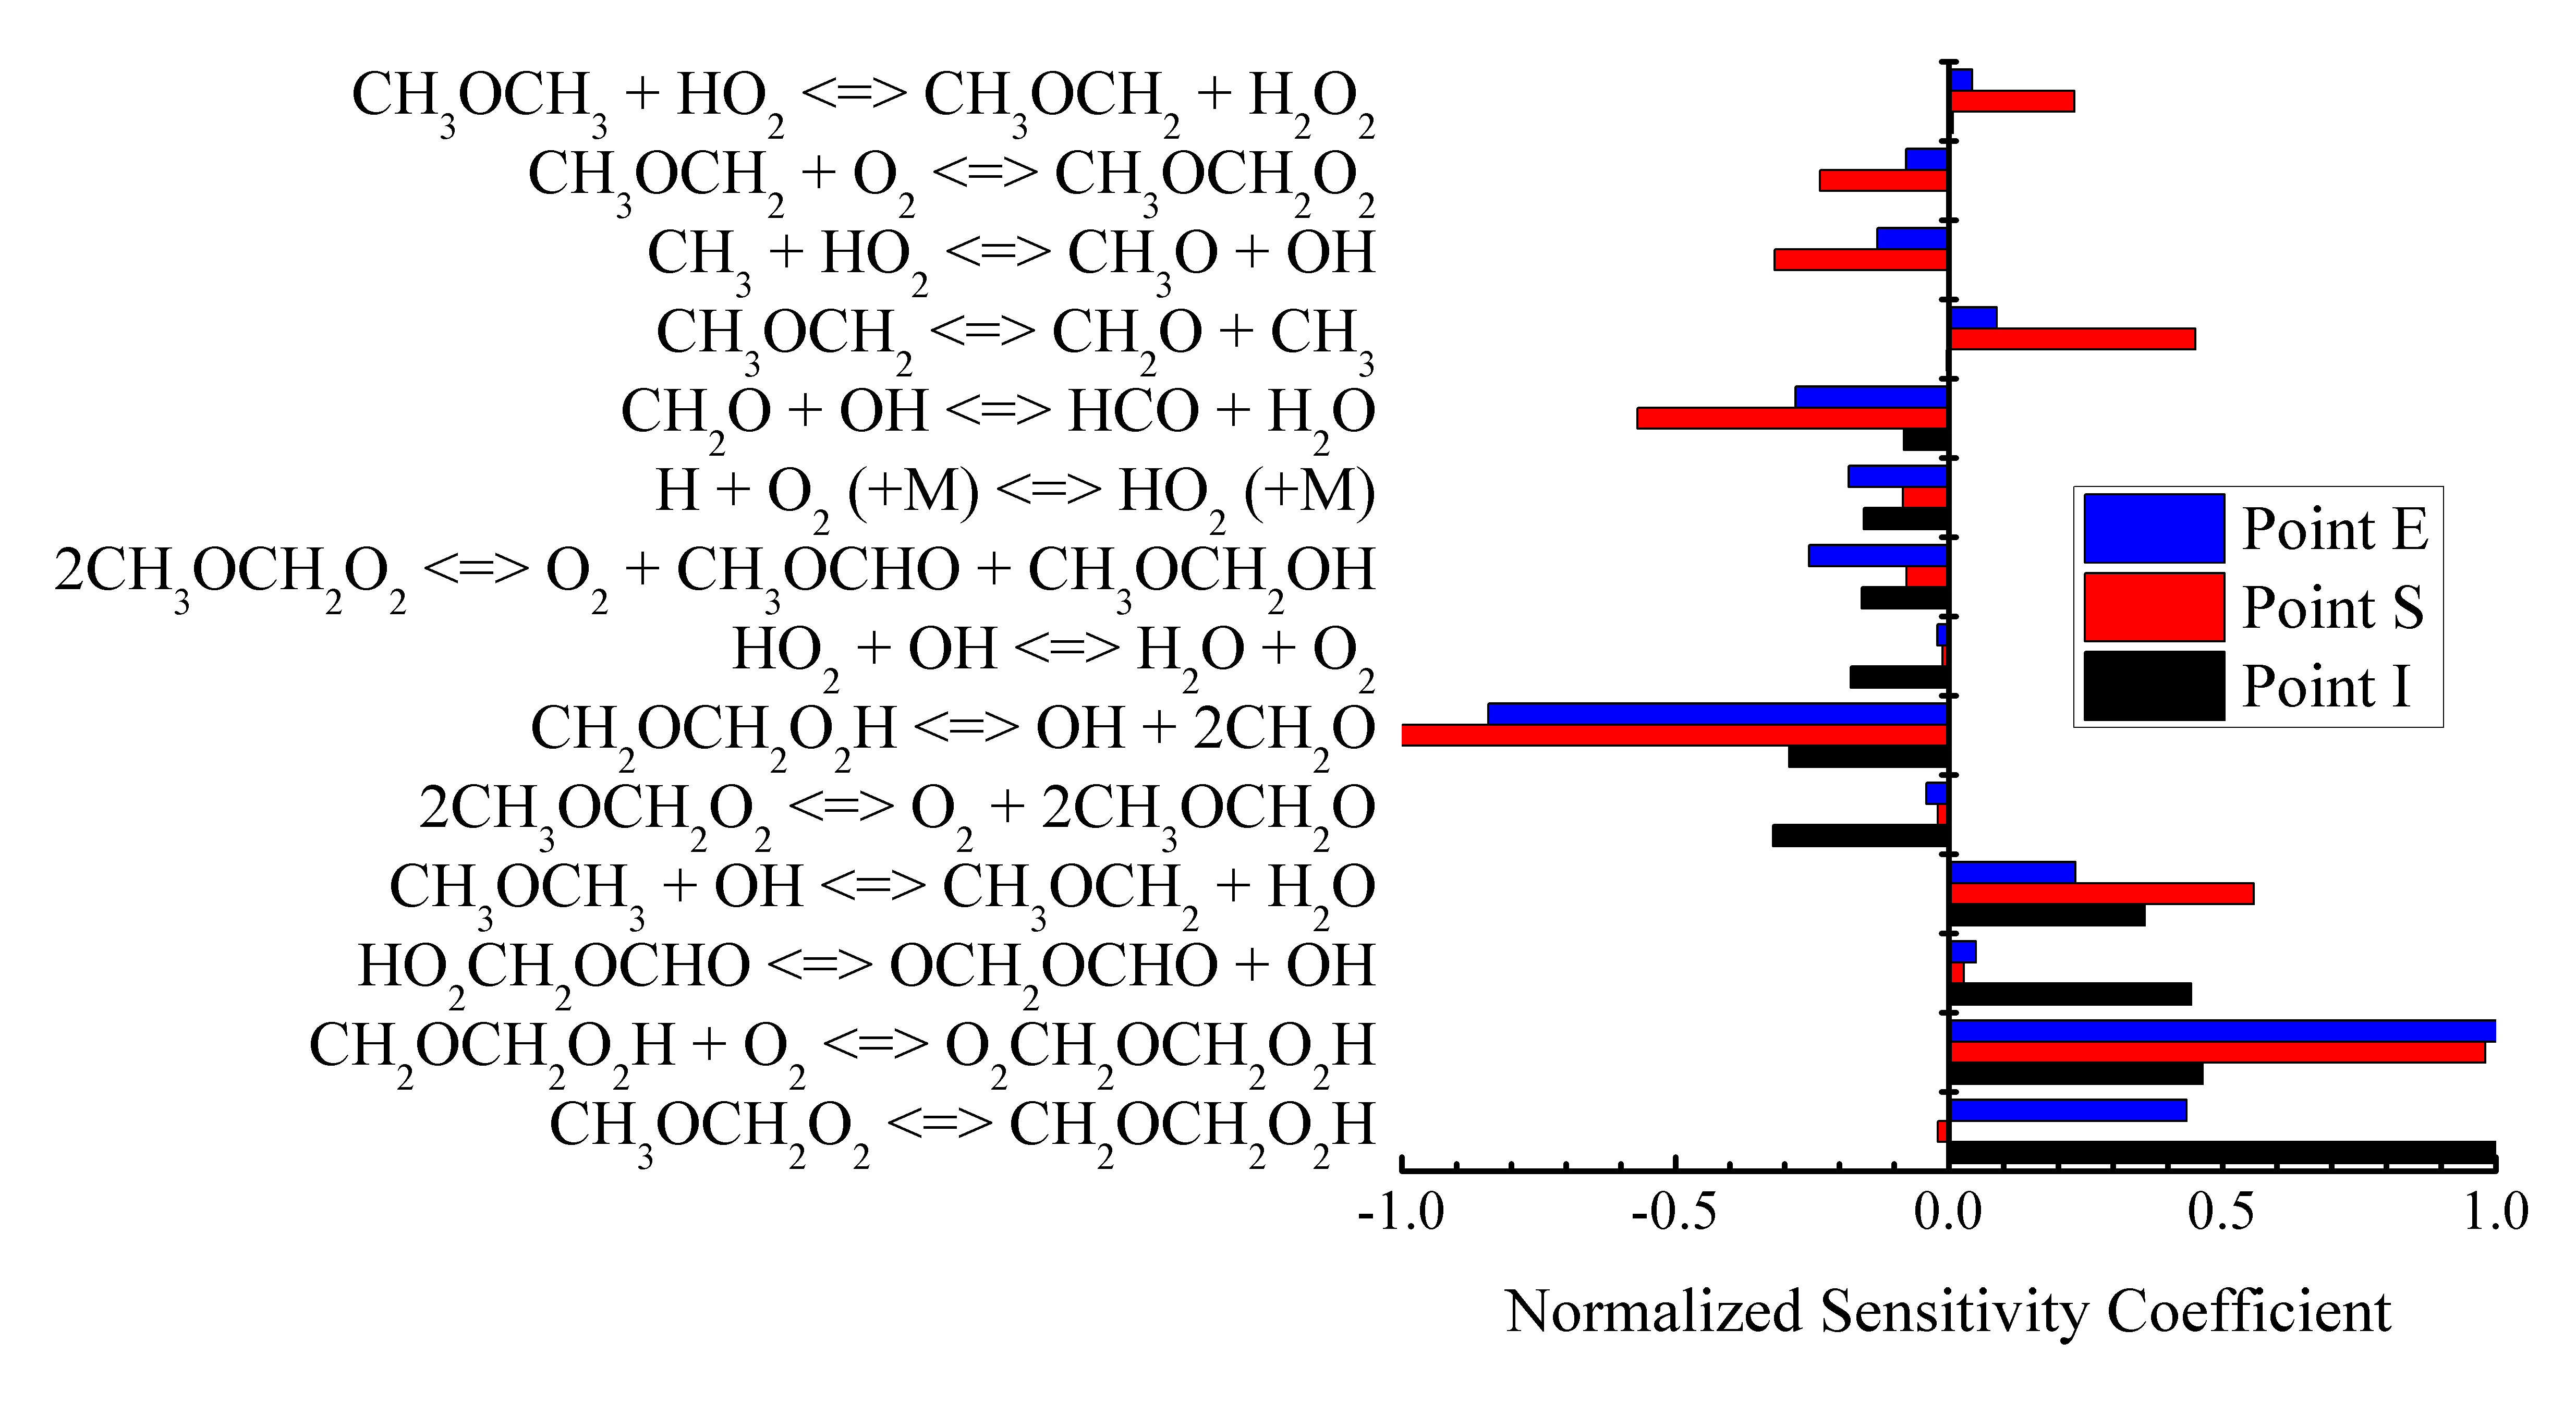
\includegraphics[width=0.5\textwidth]{SA.png}
  \normalsize
  \caption{Reaction sensitivity analysis at three representative points on the S-curve shown in Fig.~\ref{fig:S-curve}.}
  \label{fig:SA}
\end{figure*}

\clearpage

\subsection{Uncertainty analysis}\label{sec:uncertainty}

\begin{figure*}[t]
  \centering
  \scriptsize
  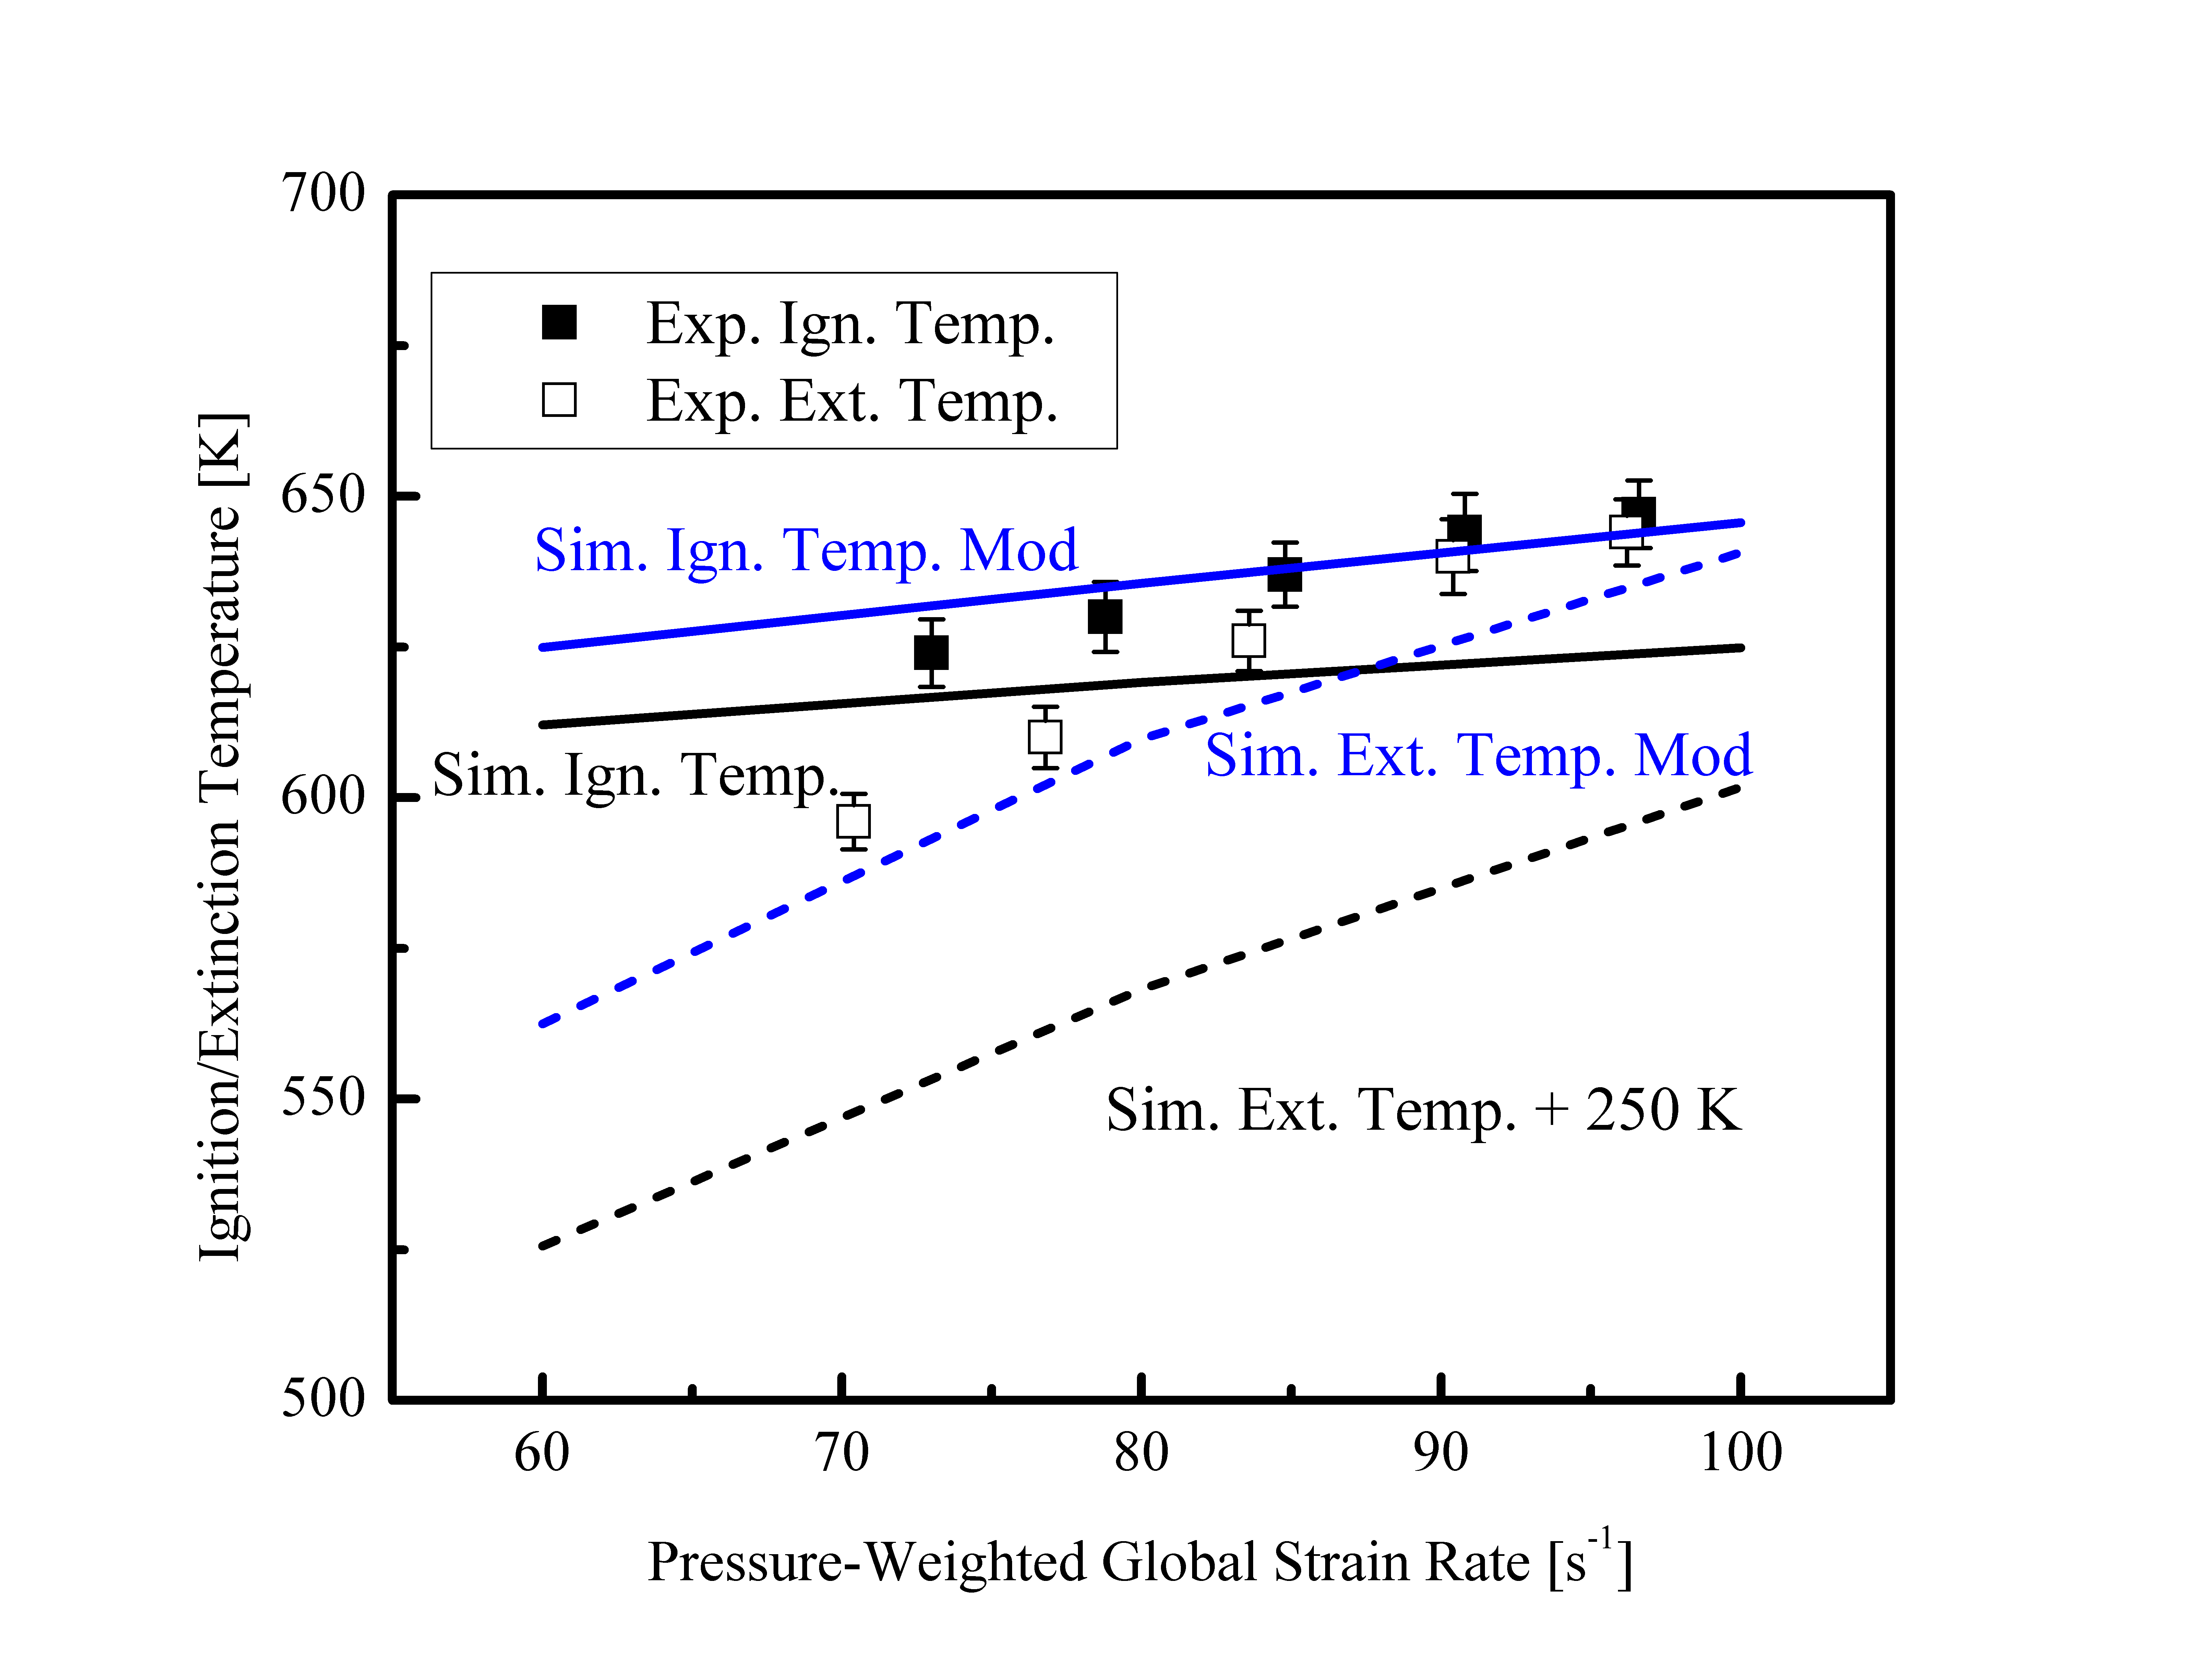
\includegraphics[trim=6.5mm 7.5mm 7mm 8mm, clip=true, width=0.5\textwidth]{cmp_demo_mod.png}
  \normalsize
  \caption{Revisit of Fig.~\ref{fig:cmp_demo} with modified reaction rates in the chemical mechanism.  Note that the line plots with the modified reaction rates are presented without shifting.}
  \label{fig:cmp_demo_mod}
\end{figure*}

As noted in Fig.~\ref{fig:cmp_demo}, while the computation is able to capture the experimental observation of the hysteretic feature of ignition and extinction, as well as the increasing trend of ignition and extinction temperatures with increasing strain rate, the quantitative agreement is rather poor.  Specifically, the ignition temperature is slightly overpredicted; its sensitivity to strain rate, indicated by the slope of the ignition temperature profile, is substantially underpredicted; and, most importantly, the extinction temperature is significantly underpredicted. Upon extensive exploration of the various experimental and modeling factors that could contribute to such substantial disagreements, the uncertainty of the low-temperature chemistry used in the computation has surfaced to be the dominant factor.

To demonstrate the effects of such uncertainty and since the ignition temperatures of the cool flames are fairly well captured, it is reasonable to inspect reactions with large sensitivity coefficients in Fig.~\ref{fig:SA} for the cool flames.  This leads to the identification of the reactions: $\rm{CH}_2\rm{OCH}_2\rm{O}_2\rm{H} + \rm{O}_2 \Longleftrightarrow \rm{O}_2\rm{CH}_2\rm{OCH}_2\rm{O}_2\rm{H}$ and $\rm{CH}_2\rm{OCH}_2\rm{O}_2\rm{H} \Longleftrightarrow \rm{OH} + 2\rm{CH}_2\rm{O}$.  Since cool flames appear to be more robust to extinguish, we have repeated the calculation by modifying the preexponential factors of these two reactions by respectively reducing and increasing to 70\% and 200\% of their original values.


Figure~\ref{fig:cmp_demo_mod} then shows that both qualitative and quantitative agreements between experiments and computations are achieved with the modified reaction parameters.  Specifically, although the magnitude of the ignition temperature is not very sensitive to the modifications, as expected, its sensitivity to increasing strain rate is enhanced, for the modifications essentially slow down the low-temperature chemistry such that the sensitivity to finite residence time is more pronounced.  More importantly, it is seen that good agreement is also achieved for the highly sensitive extinction temperatures, significantly boosting their values but without changing the sensitivity to the strain rate variation.

\textcolor{Rev1}{While the above results appear to be encouraging, we hasten to clarify that we are not suggesting modified kinetic parameters for certain reactions. What we have demonstrated is the sensitive nature and potential uncertainty of the low-temperature chemistry, in that substantial change in the global response can result from even small changes in these preexponential factors.}  \textcolor{Rev2}{We noted that although the Zhao \emph{et al.} model, which the adopted skeletal model was based on, was still the most well accepted, more experimental data had become available recently to guide the modifications of the low-temperature chemical pathways and kinetic parameters in the models~\cite{burke15,rodriguez15}.  However, we further note that, during the development of the low-temperature chemical model, the validation data is limited to those from homogeneous systems.  The current study aims at providing validation targets in inhomogeneous systems by substantiating the existence of the nonpremixed cool flame and revealing the evolution of low-temperature chemistry during ignition and extinction processes.  Clearly, additional validation data on cool flames covering a wider range of conditions, which are inherently present in flame systems, is needed from the community.}

Another factor that could potentially affect the accuracy of the comparison between the experimental and computational results is the experimental detection limit of the UV camera, which could be too high compared to the chemiluminescence emission of the cool flame near extinction.  Since the hysteresis temperature window was observed in the experiment at various conditions, the detection threshold of the UV camera should be lower than the chemiluminescence intensity of the steady cool flame upon ignition.  Consequently, the ignition temperatures for these cases should be well captured.  However, the lower bound of the hysteresis temperature window could be limited by the detection threshold, and therefore, the actual extinction temperatures might not be captured accurately.

%\textcolor{Rev2}{Shan and Lu conducted a computational study on ignition and extinction of DME/air mixture at high pressure in a perfectly stirred reactor (PSR).

\subsection{Effects of pressure and oxygen concentration}

\begin{figure*}[t]
  \centering
  \scriptsize
  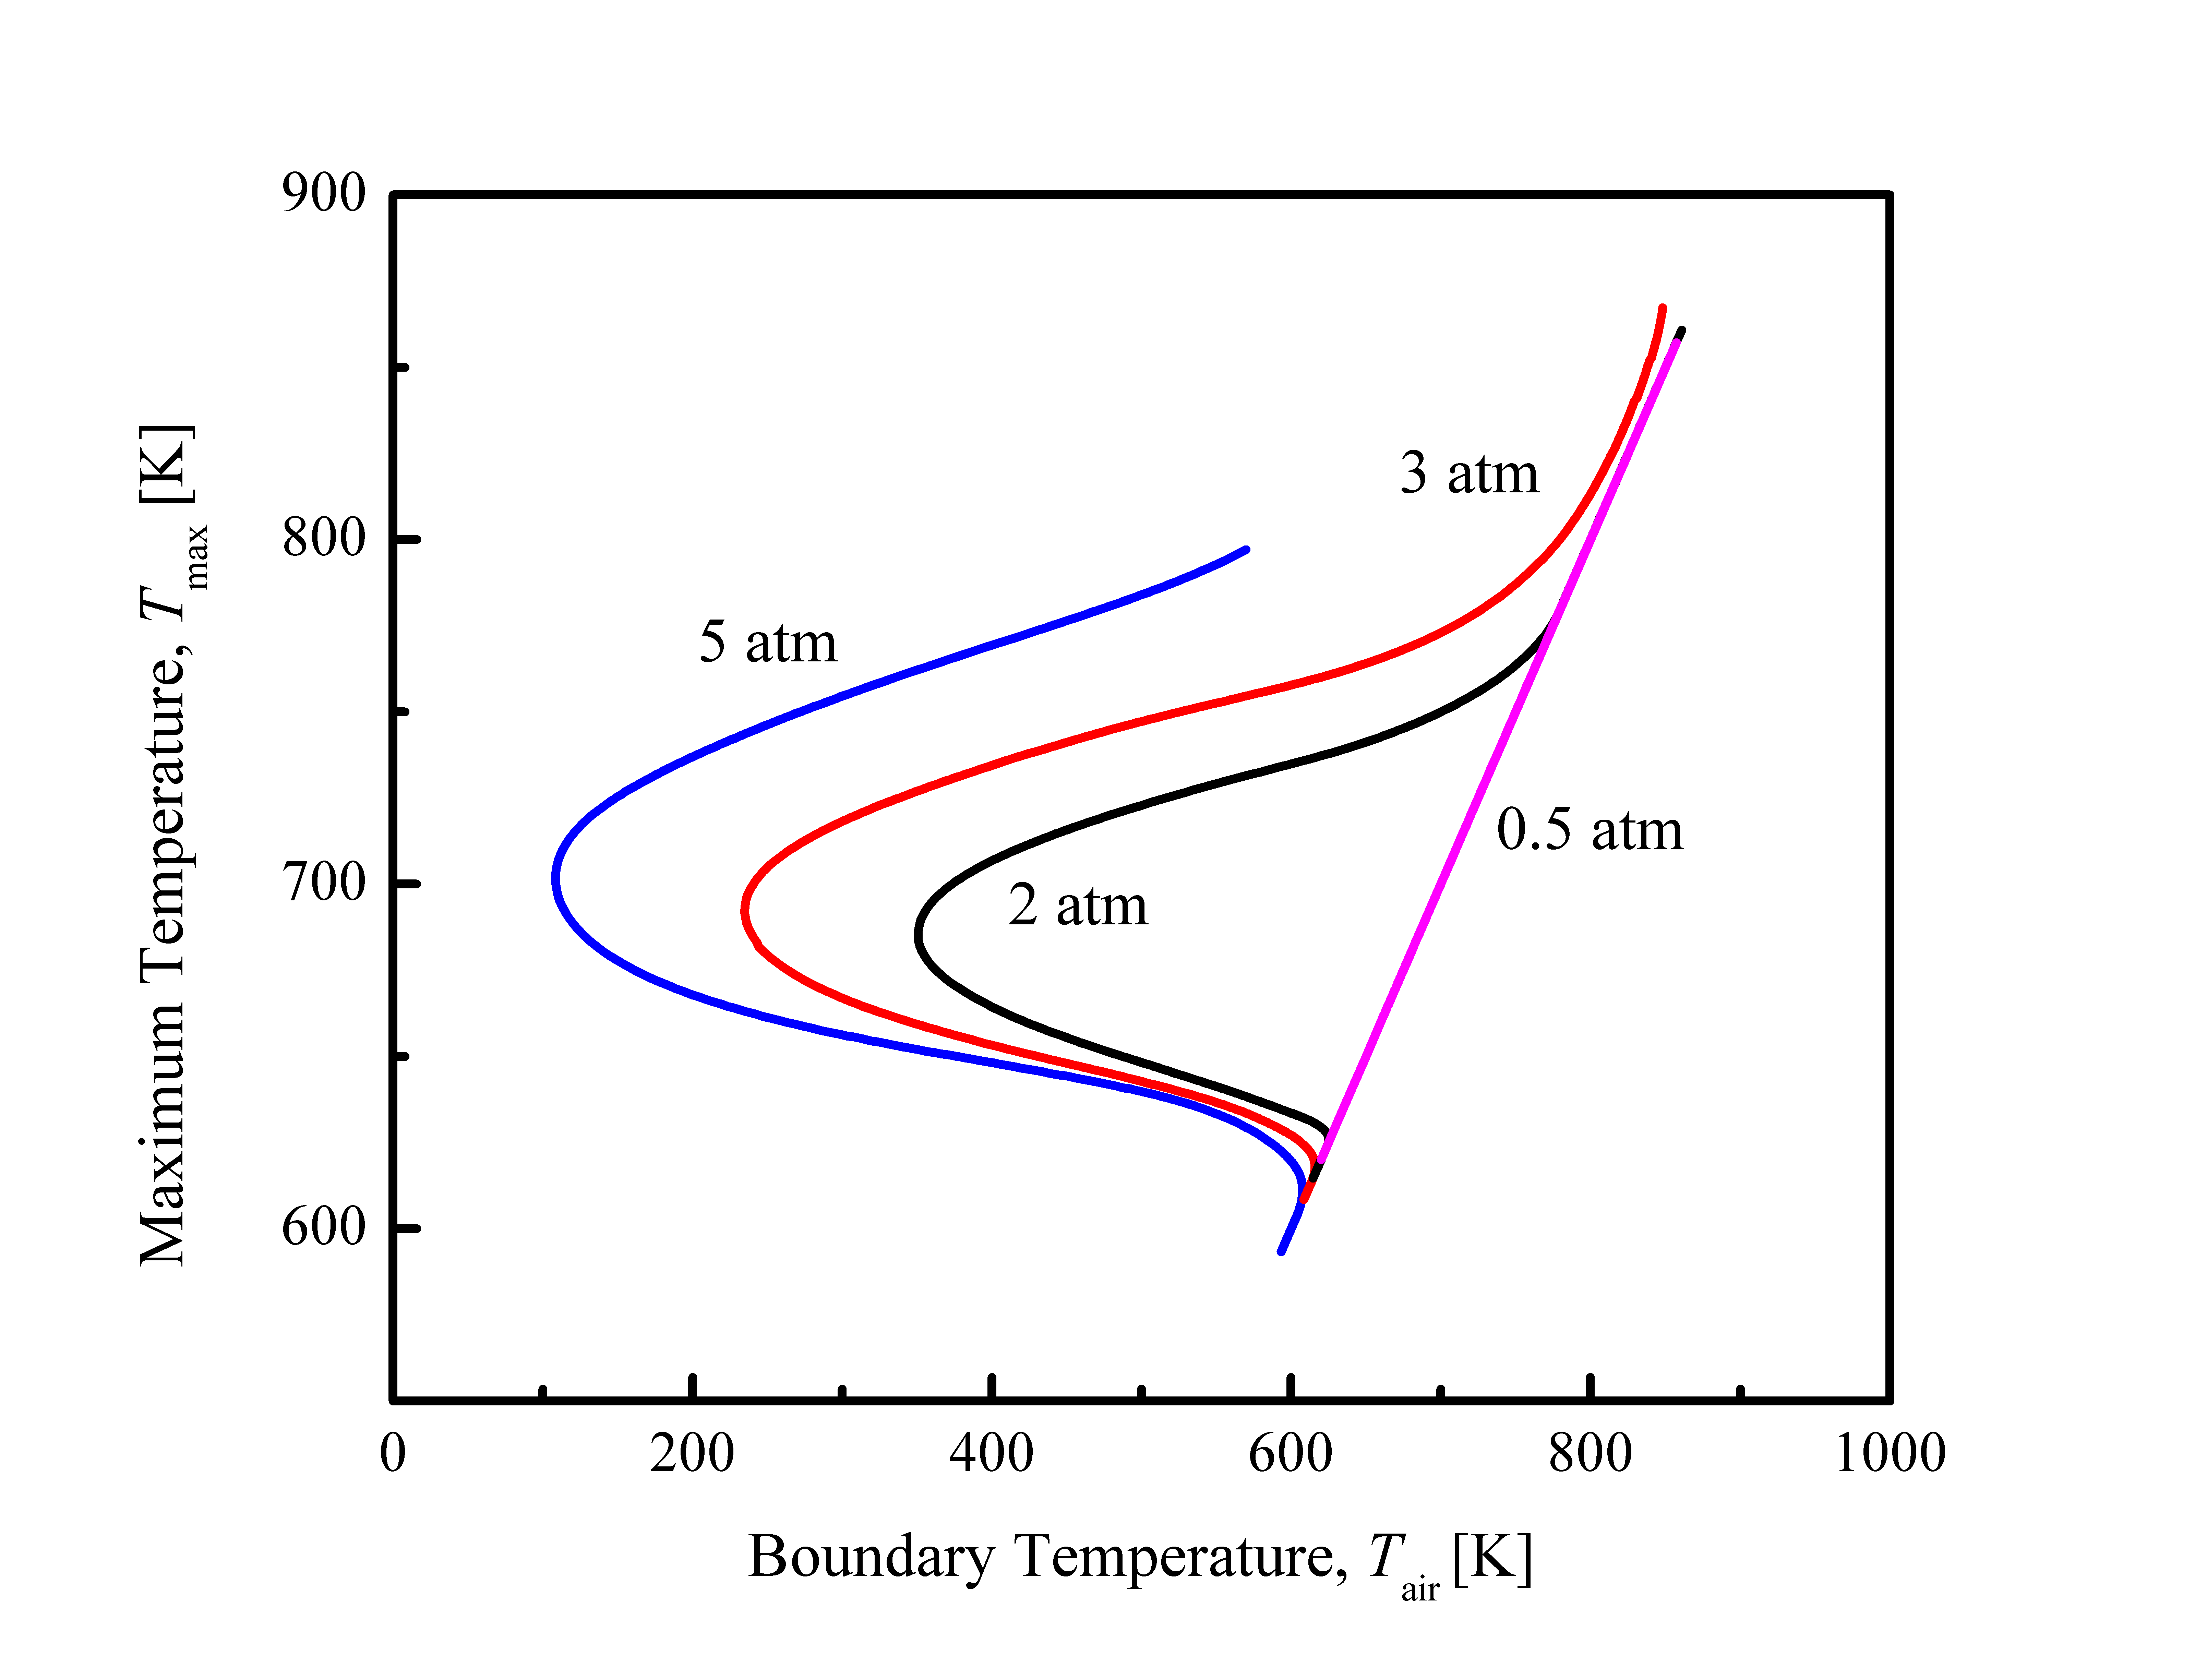
\includegraphics[trim=6.5mm 7.5mm 7mm 8mm, clip=true, width=0.5\textwidth]{eff_P.png}
  \normalsize
  \caption{S-curve analysis for various ambient pressures and pressure-weighted strain rate of 100 /s.  DME volume fraction in the fuel stream is 50\%, and the oxidizer stream is air.}
  \label{fig:eff_P}
\end{figure*}

\begin{figure*}[t]
  \centering
  \scriptsize
  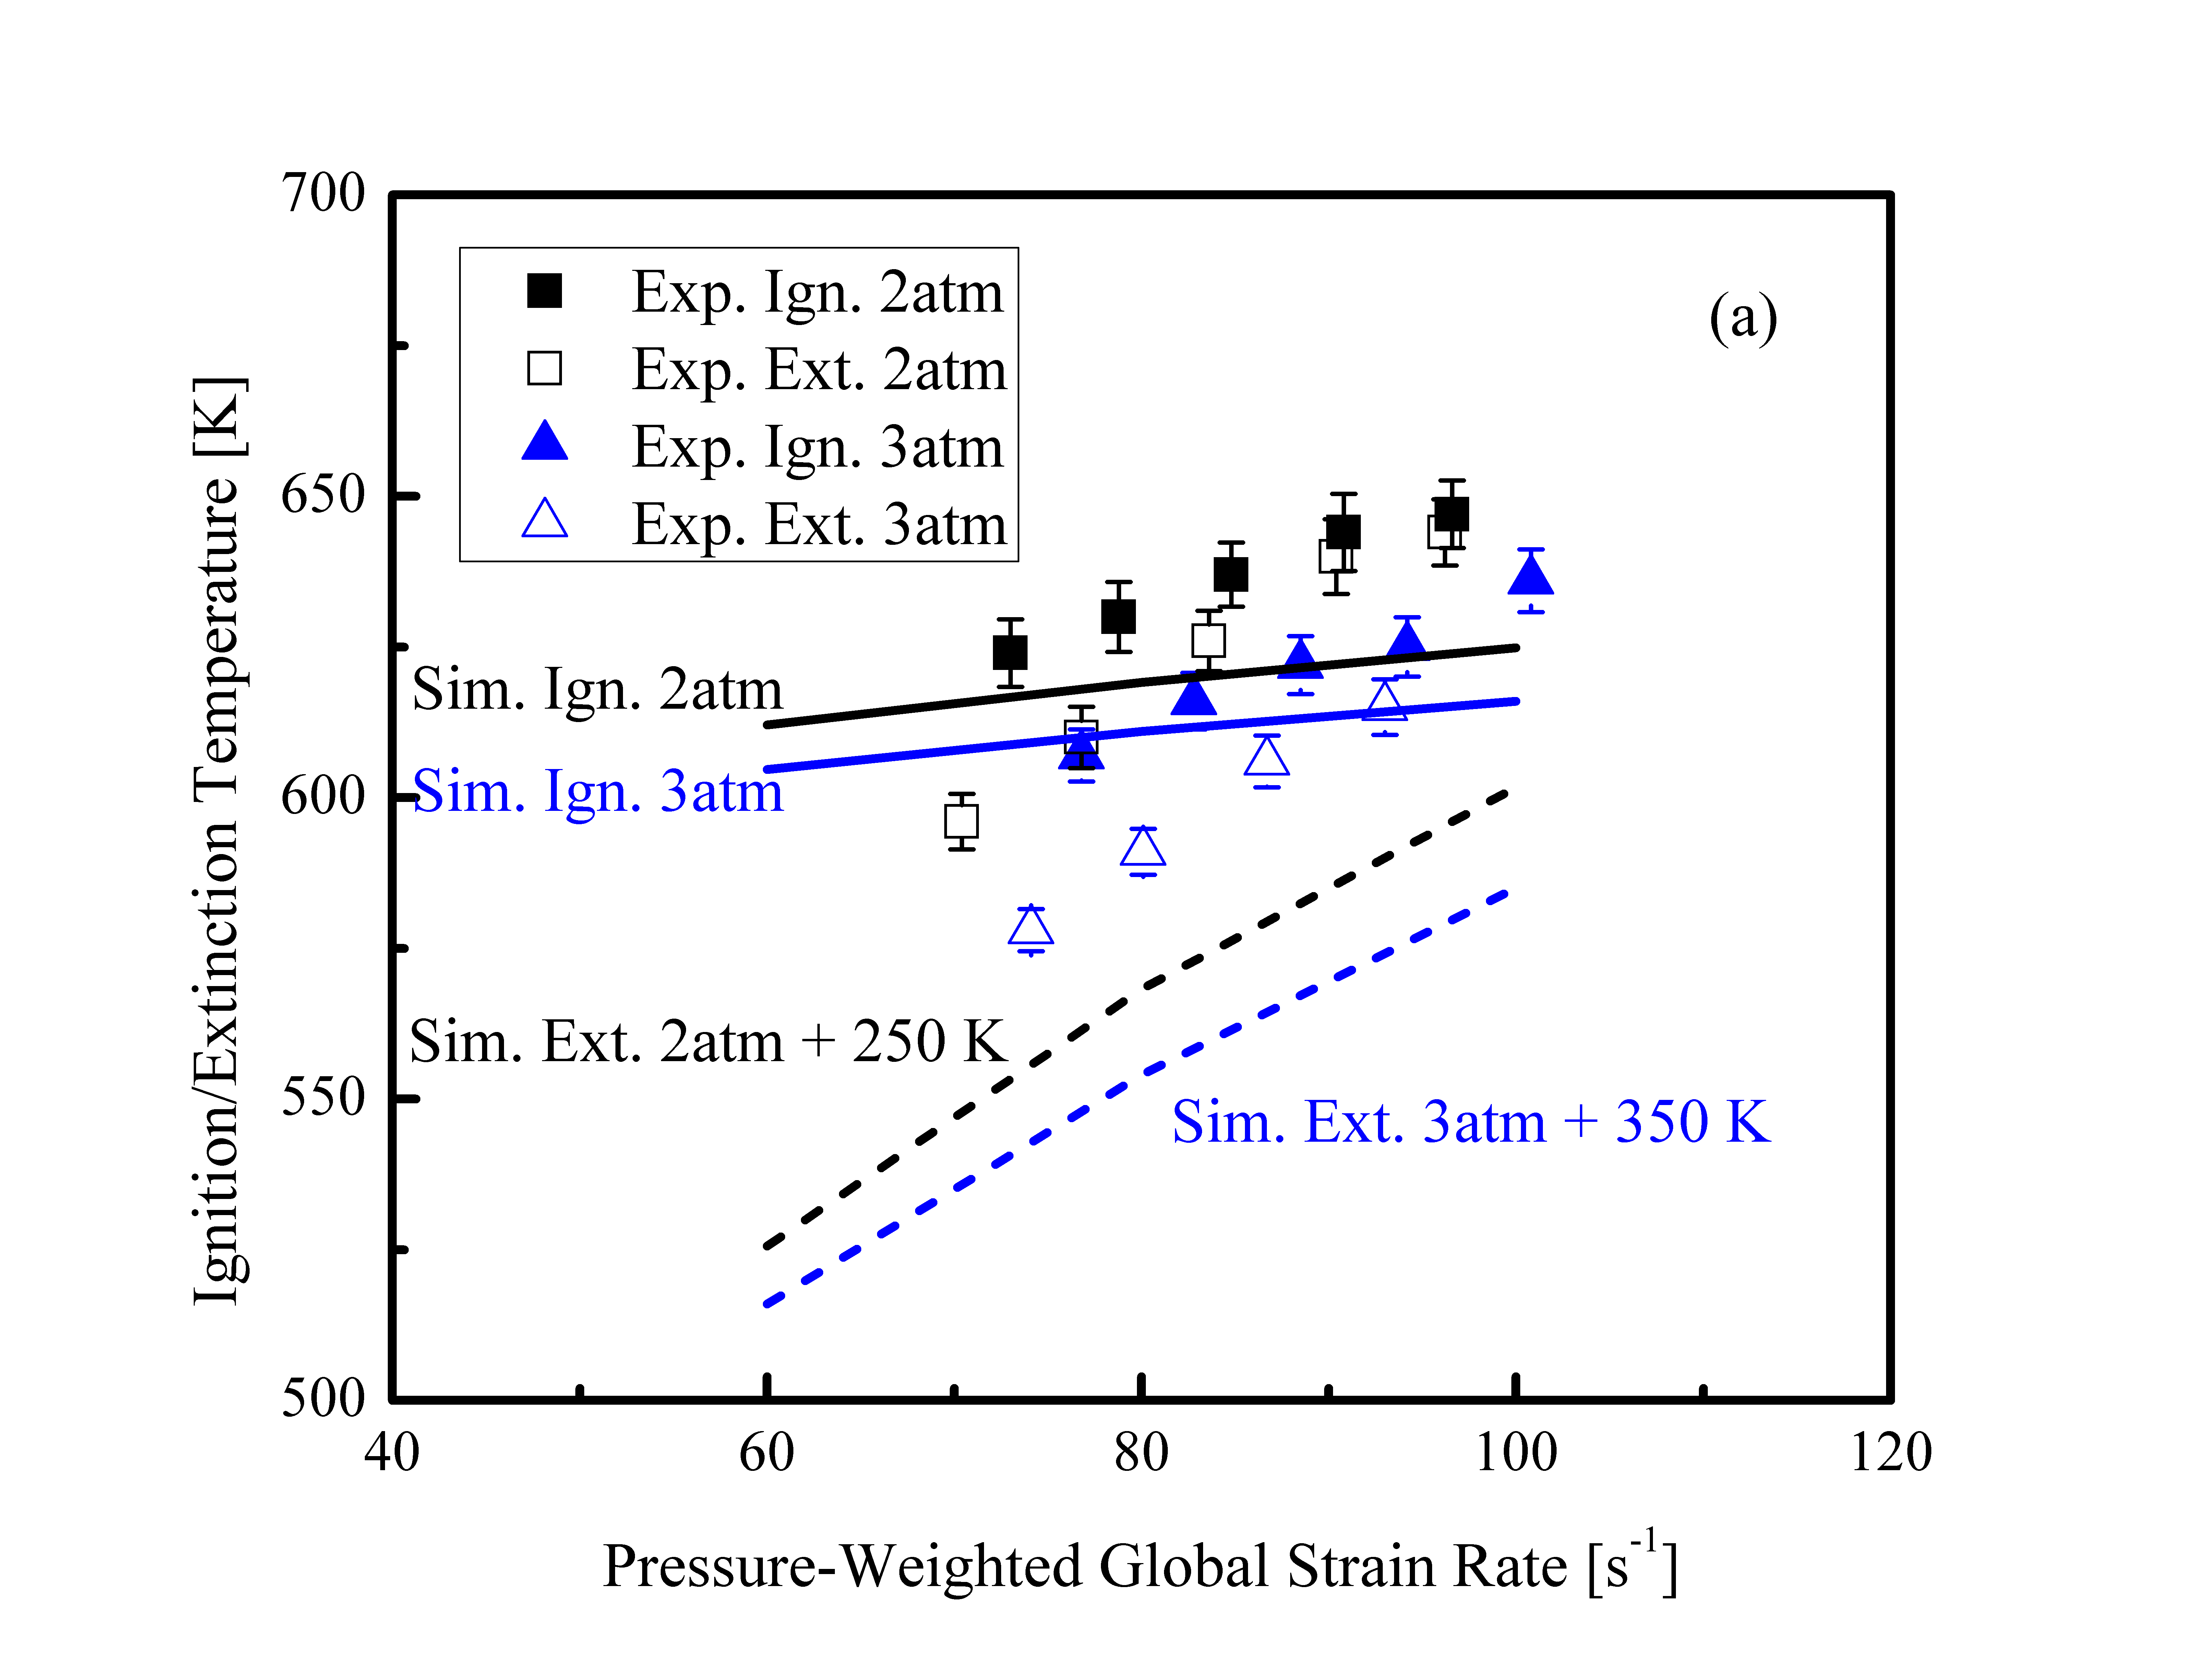
\includegraphics[trim=6.5mm 7.5mm 7mm 8mm, clip=true, width=0.5\textwidth]{cmp_P.png}
  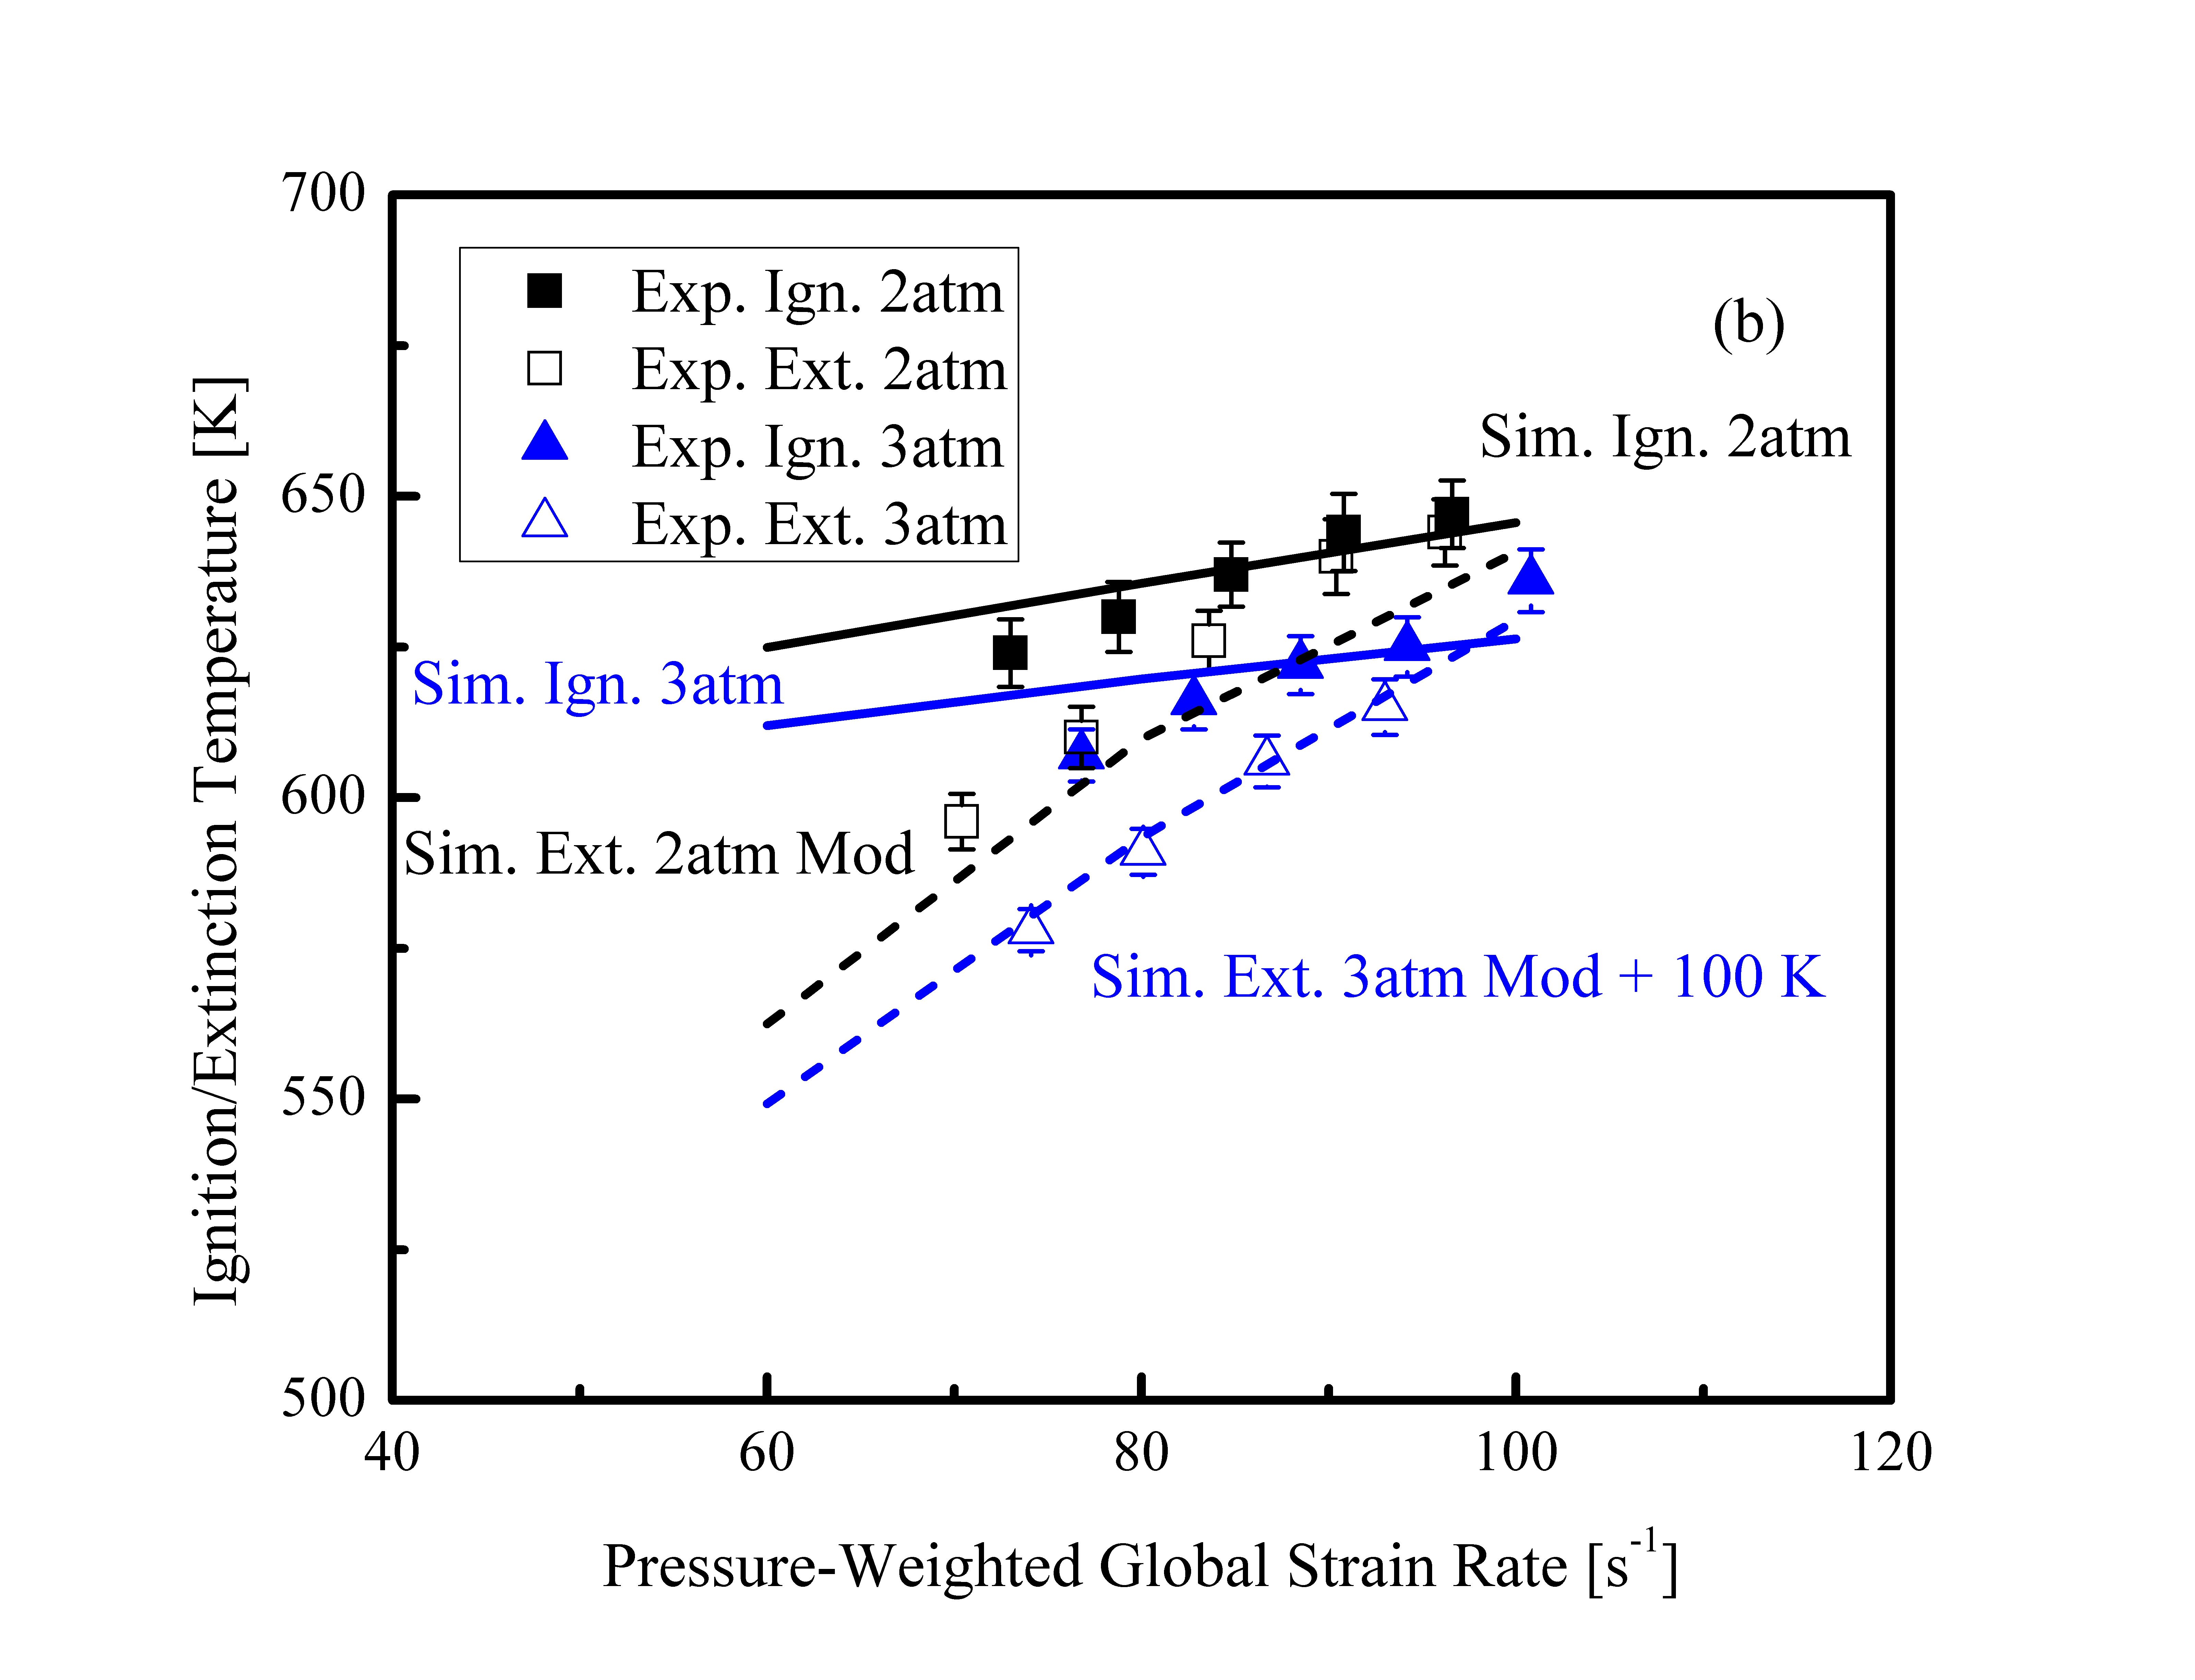
\includegraphics[trim=6.5mm 7.5mm 7mm 8mm, clip=true, width=0.5\textwidth]{cmp_P_mod.png}
  \normalsize
  \caption{Ignition and extinction temperatures at various strain rates and pressures in experiments and computations with (a) the original and (b) modified chemical models.  Some of the computed extinction temperatures are shifted up for better illustration.  DME volume fraction in the fuel stream is 50\%, and the oxidizer stream is air.}
  \label{fig:cmp_P}
\end{figure*}

\begin{figure*}[t]
  \centering
  \scriptsize
  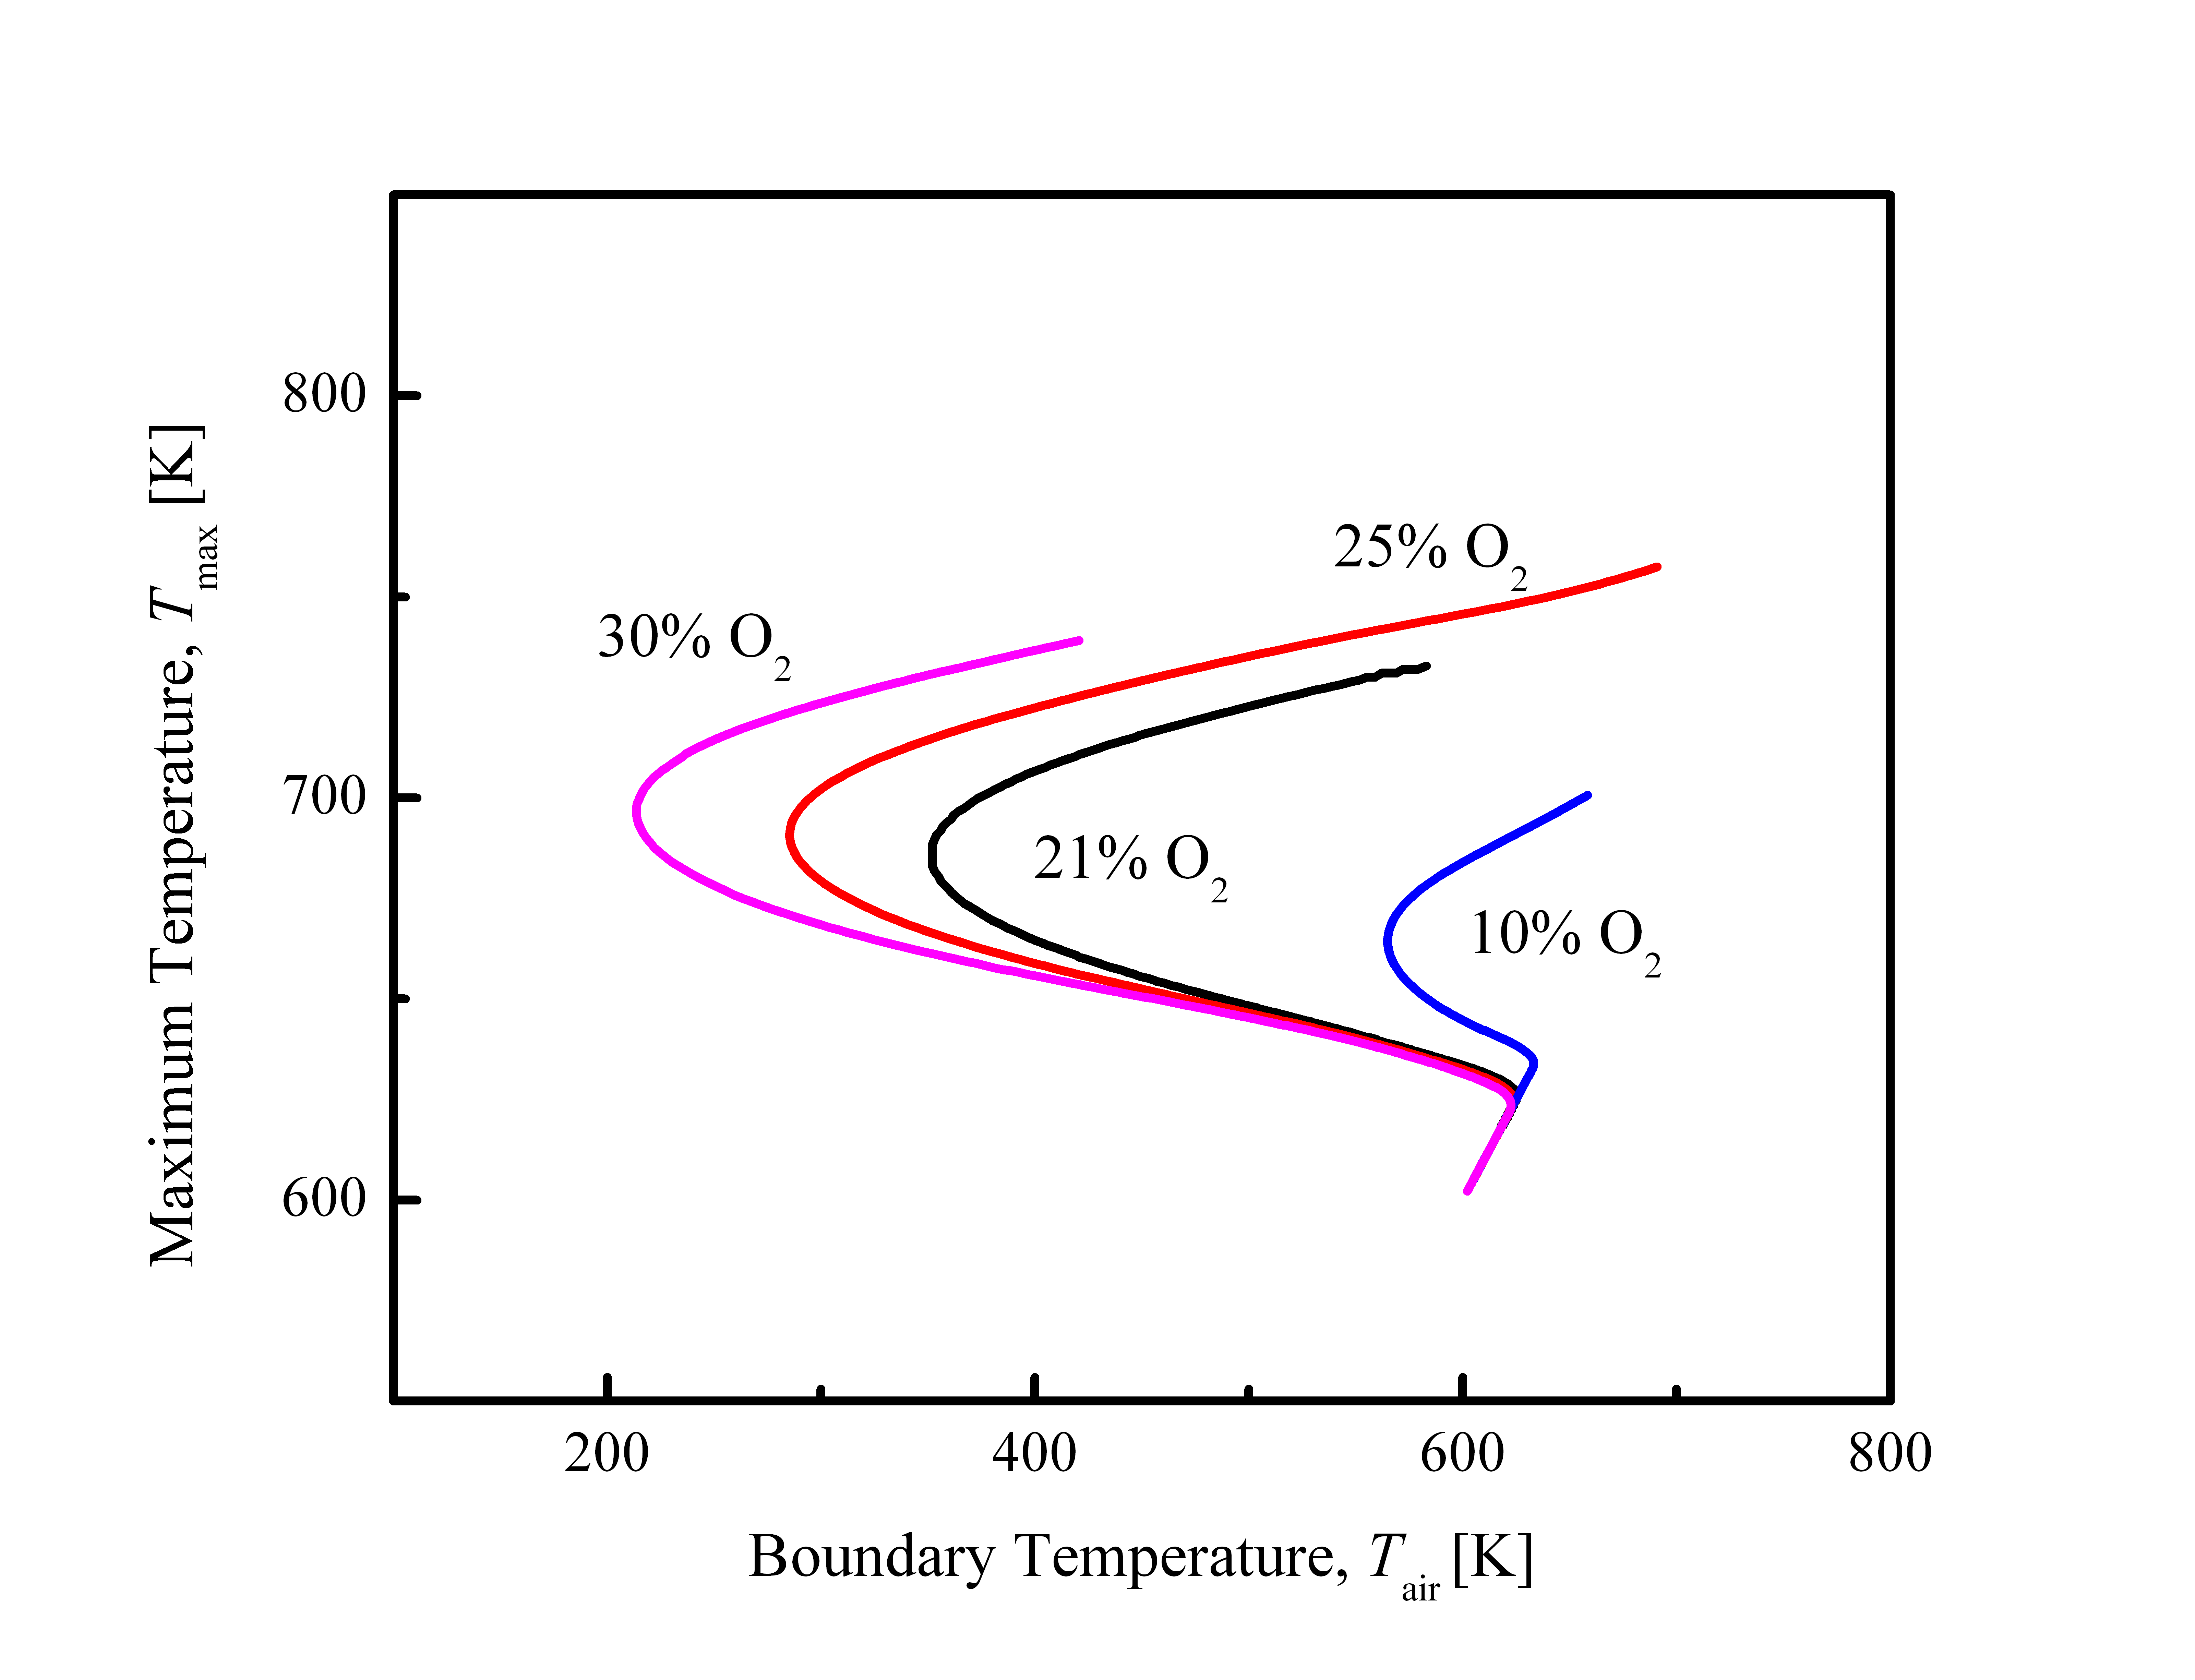
\includegraphics[trim=6.5mm 7.5mm 7mm 8mm, clip=true, width=0.5\textwidth]{eff_O2.png}
  \normalsize
  \caption{S-curve analysis for various oxygen concentrations and the pressure-weighted strain rate of 100 /s.  DME volume fraction in the fuel stream is 50\%, and the ambient pressure is 2 atm.}
  \label{fig:eff_O2}
\end{figure*}

\begin{figure*}[t]
  \centering
  \scriptsize
  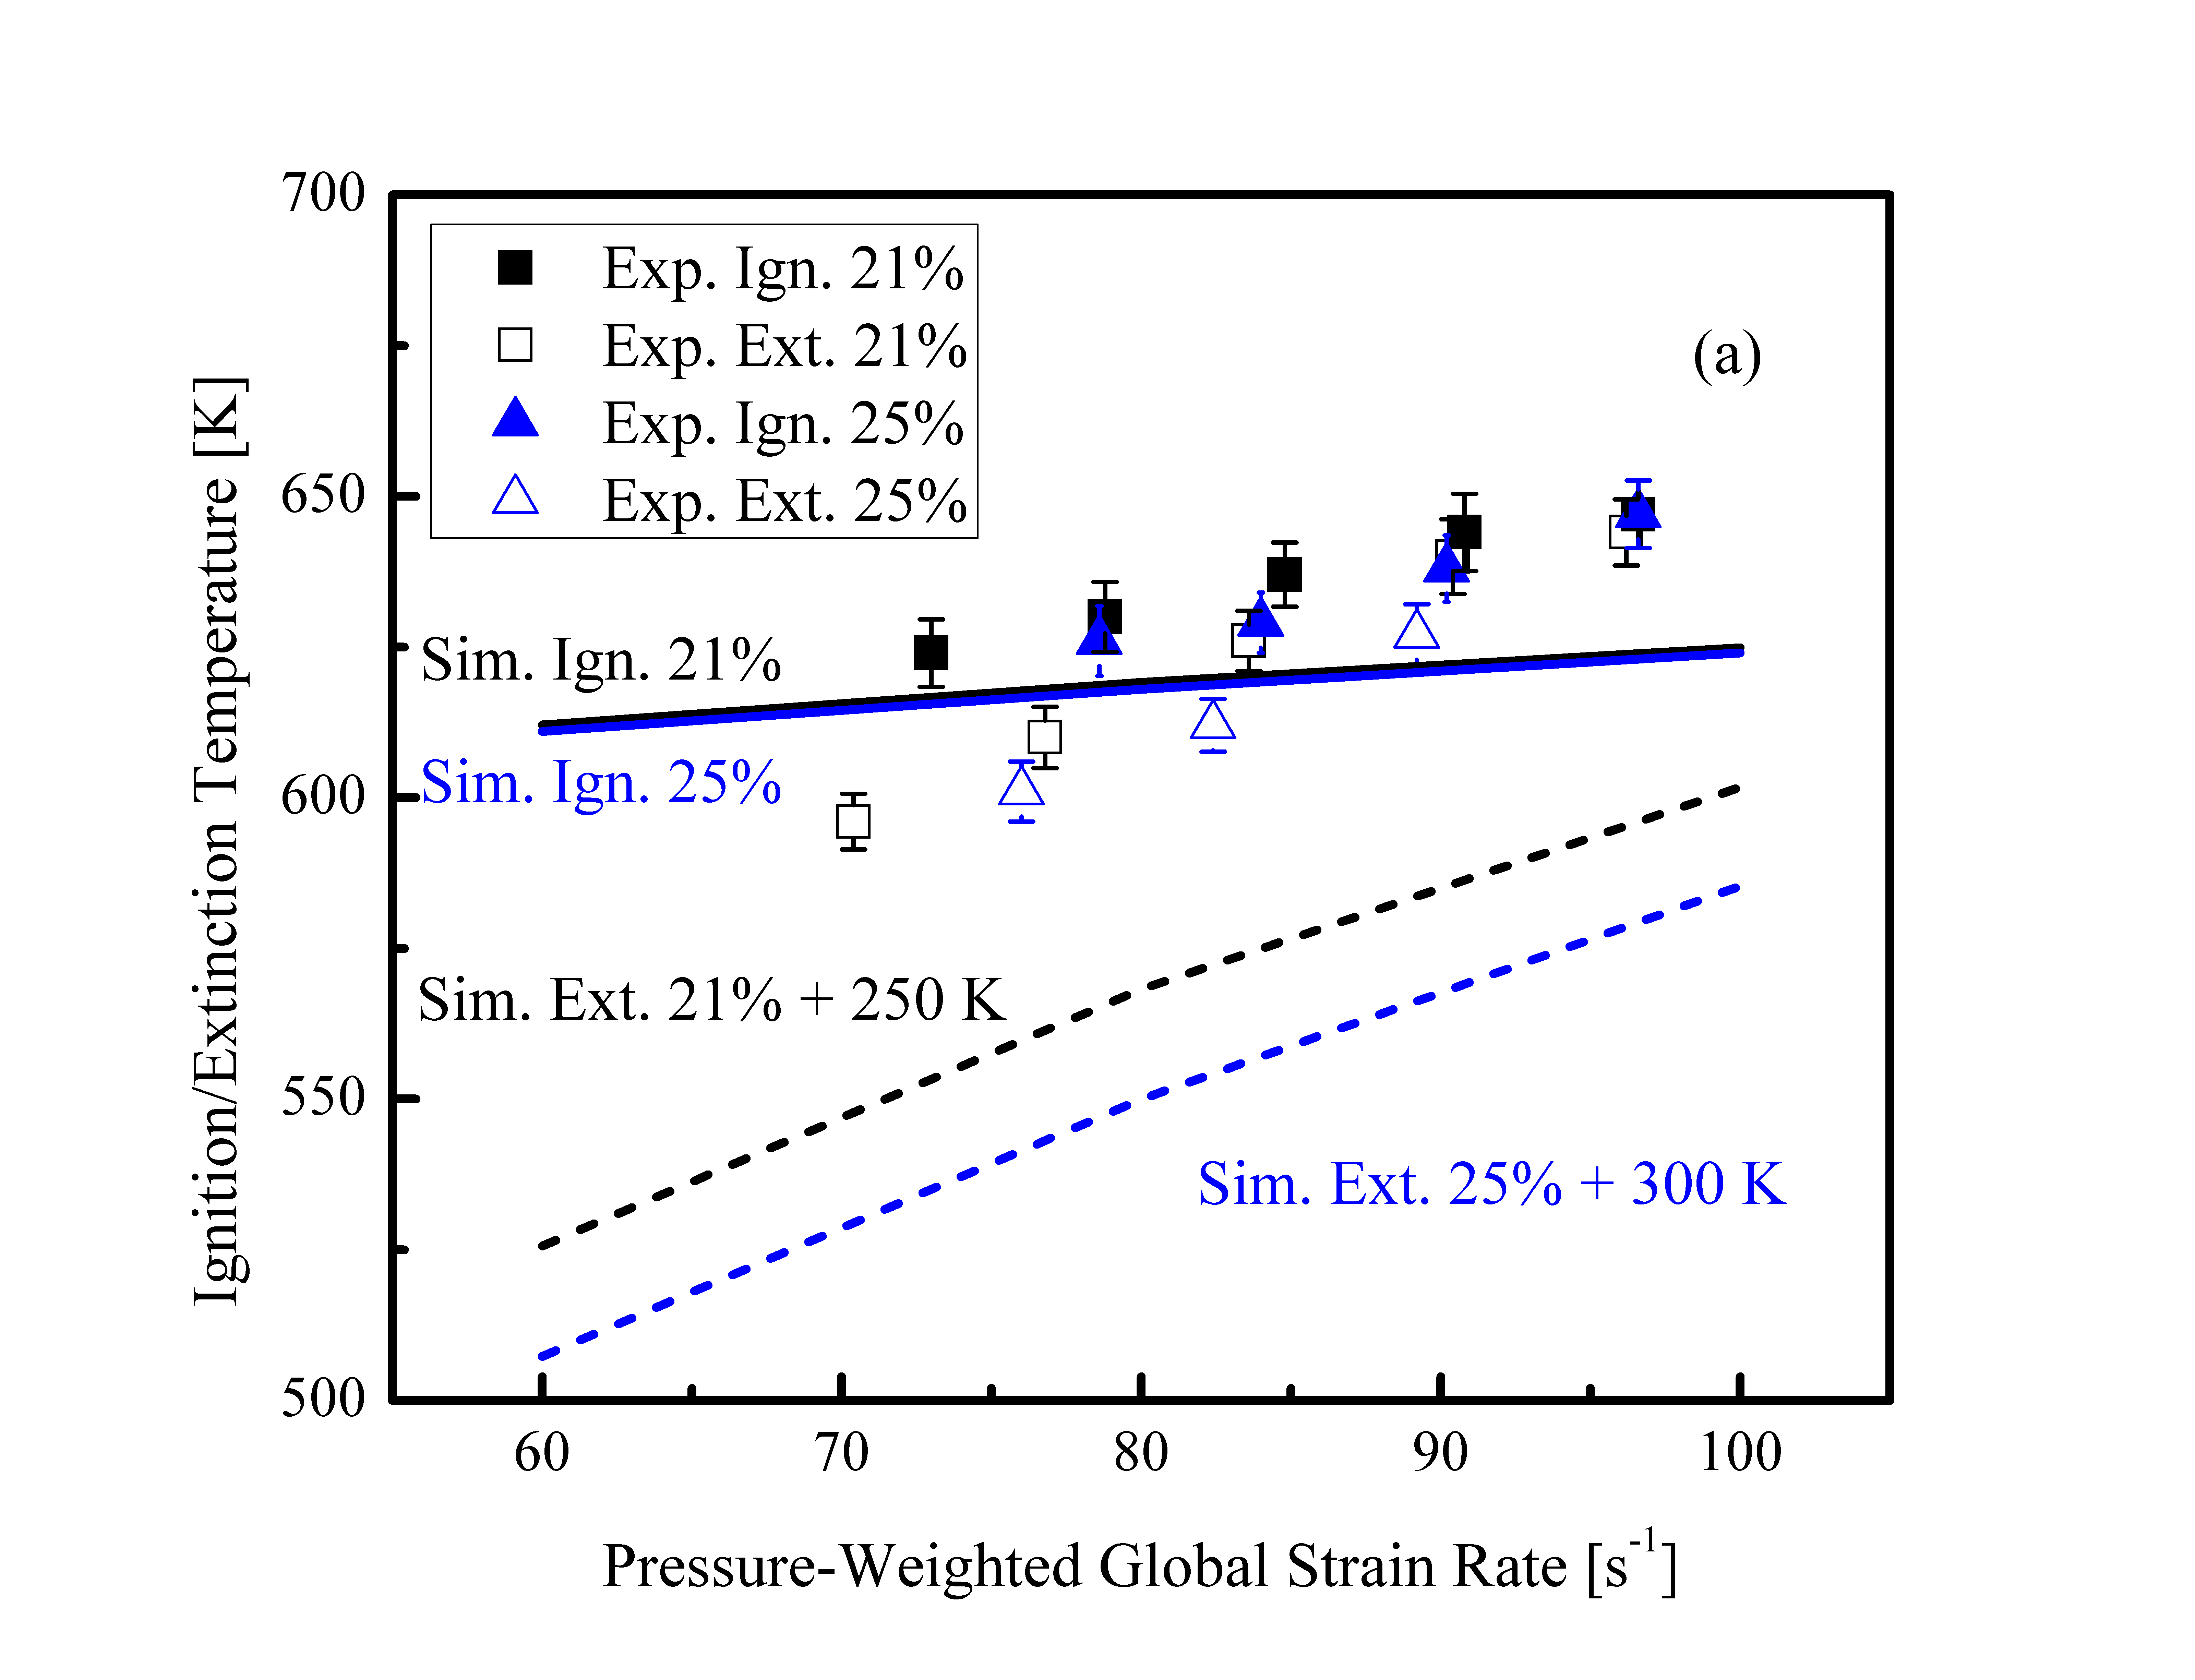
\includegraphics[trim=6.5mm 7.5mm 7mm 8mm, clip=true, width=0.5\textwidth]{cmp_O2.png}
  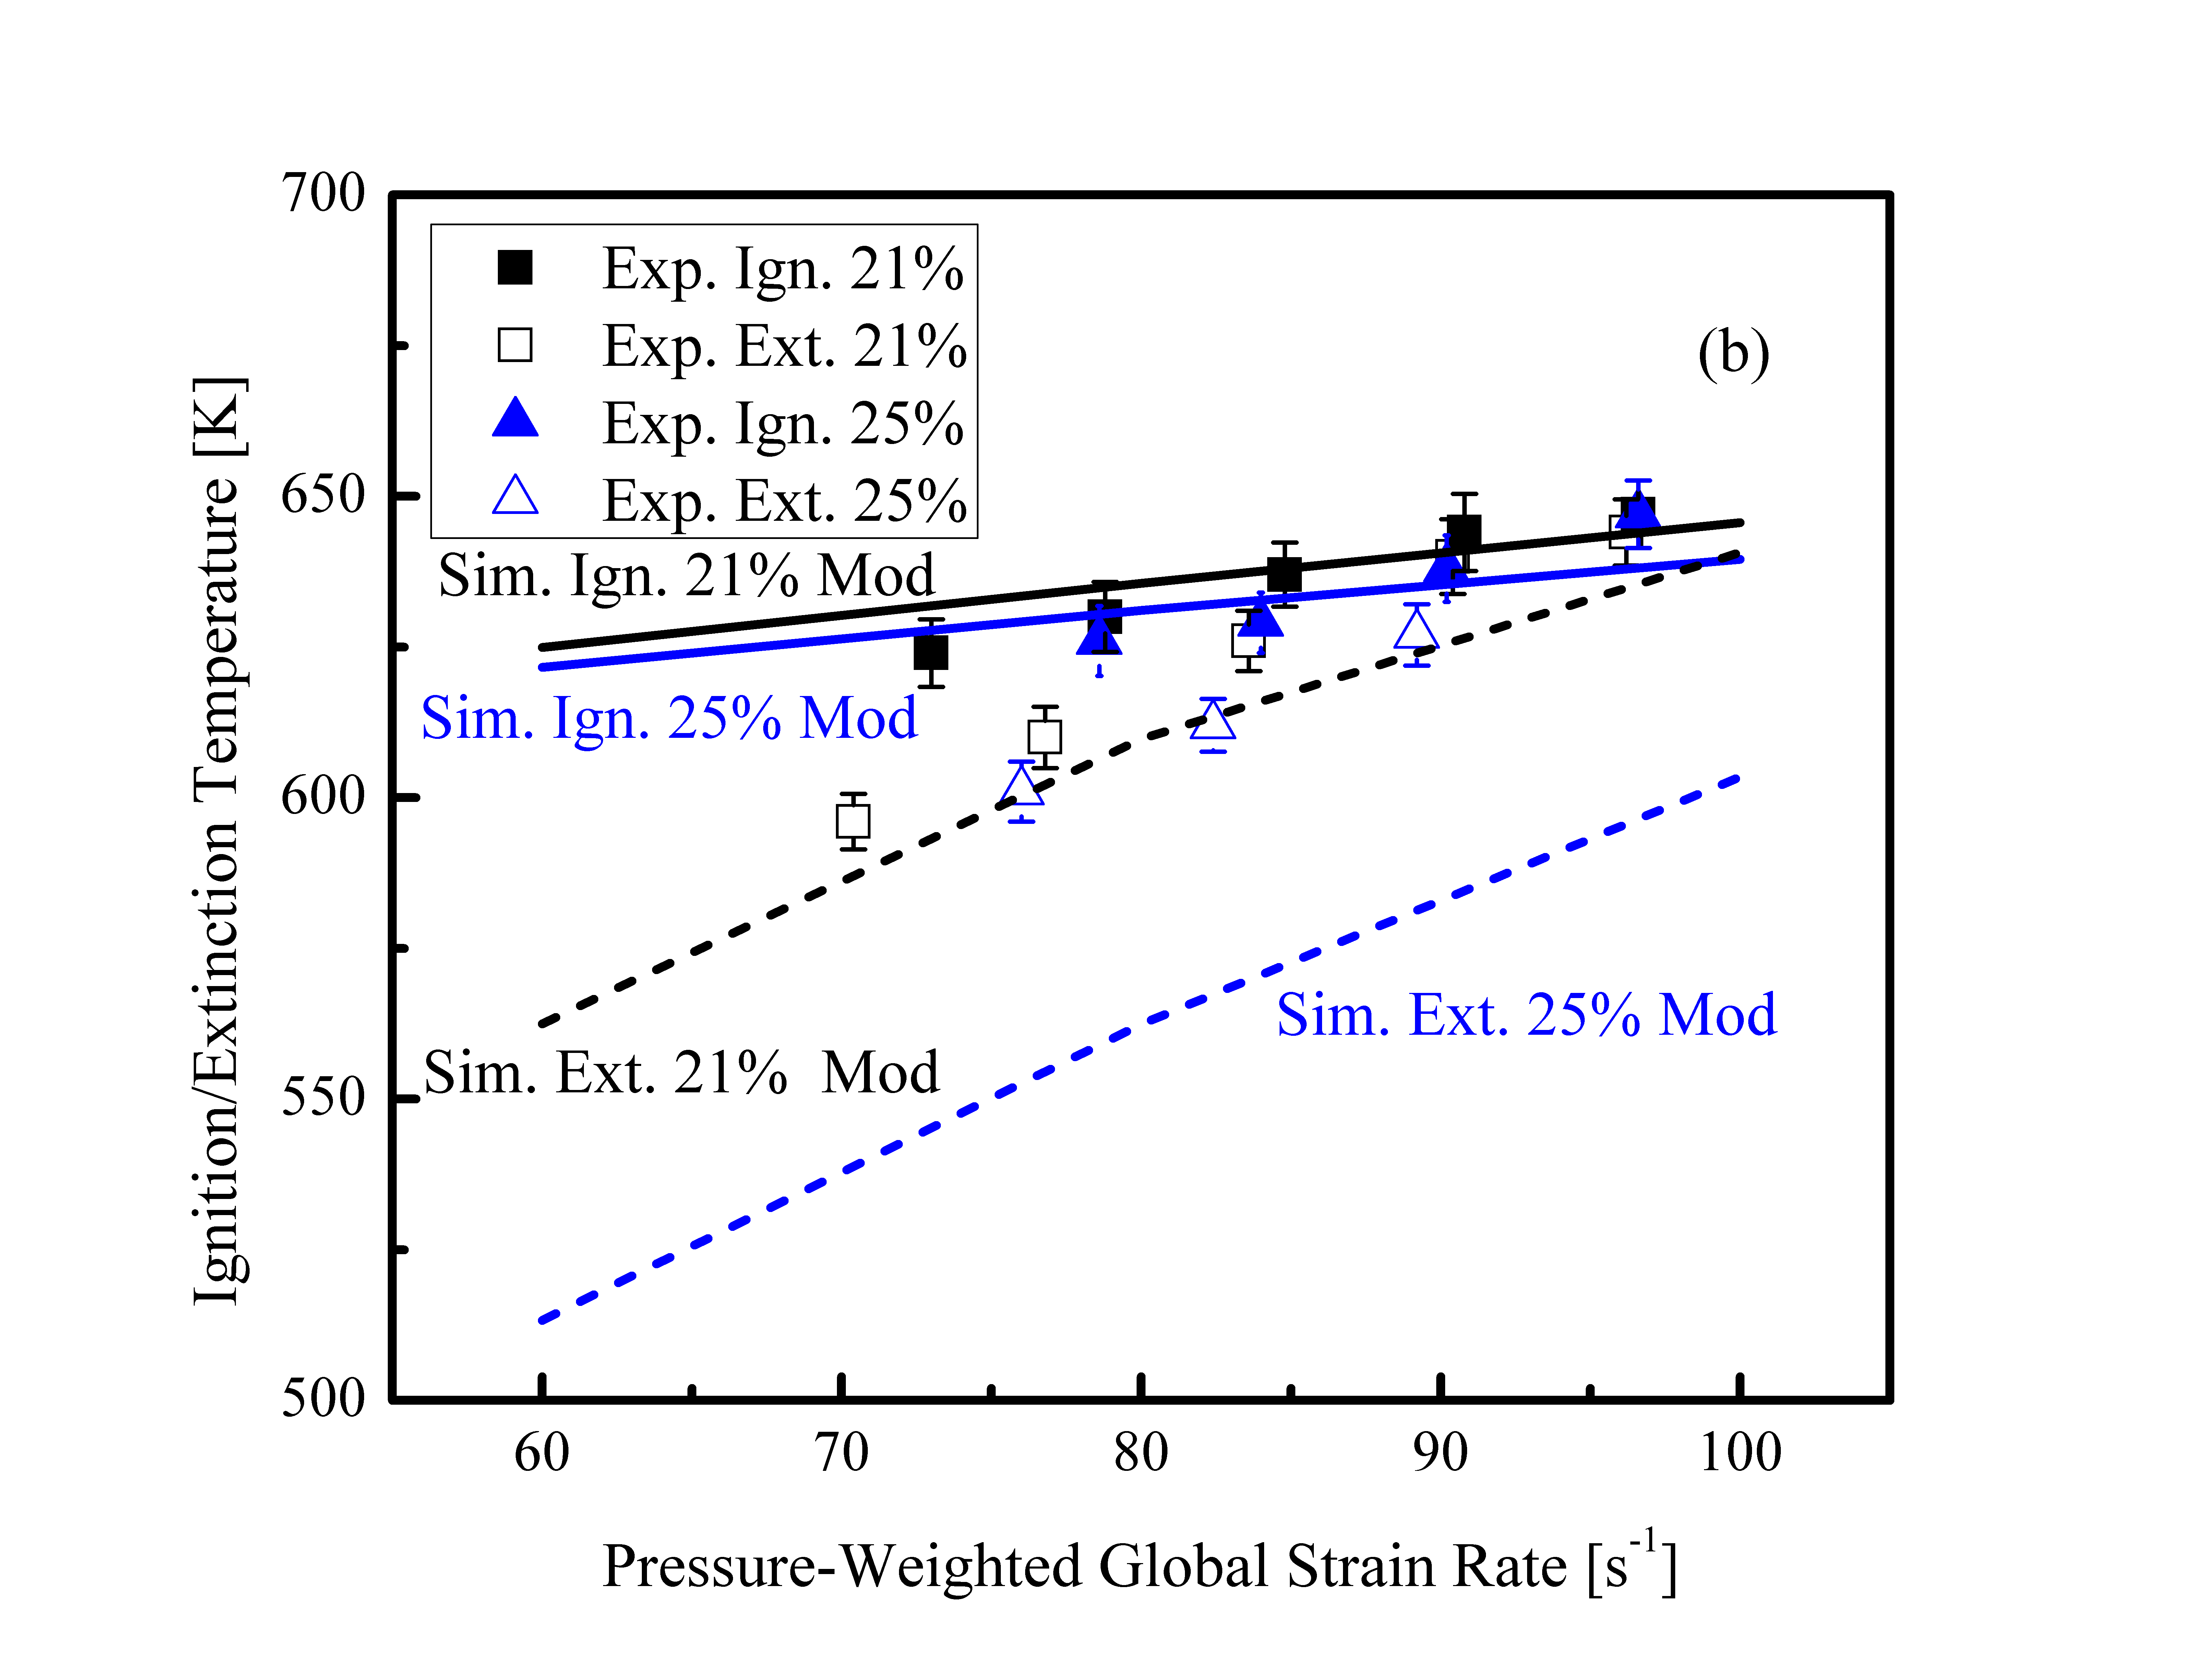
\includegraphics[trim=6.5mm 7.5mm 7mm 8mm, clip=true, width=0.5\textwidth]{cmp_O2_mod.png}
  \normalsize
  \caption{Ignition and extinction temperatures at various strain rates and oxygen concentrations in experiments and computations with (a) the original and (b) modified chemical models.  Some of the computed extinction temperatures are shifted up for better illustration.  DME volume fraction in the fuel stream is 50\%, and the ambient pressure is 2 atm.}
  \label{fig:cmp_O2}
\end{figure*}


The effects of ambient pressure and oxygen concentration in the oxidizer stream on the ignition and extinction of the cool flames were also investigated.  Pressure effects were first computationally studied by fixing the oxygen mole fraction in the oxidizer stream at 21\% and fixing the pressure-weighted strain rate at 100 /s, as shown in Fig.~\ref{fig:eff_P}.  It is seen that, as the pressure increases from 2 to 5 atm, the ignition temperature decreases and the heat release from the cool flame becomes more pronounced, as indicated by the temperature differences between the ignition turning point and the point on the cool flame branch with the same boundary temperature.  Moreover, the extinction turning point shifts to a lower boundary temperature, resulting in an extended hysteresis temperature window.  Conversely, the extent of the low-temperature chemistry governed S-curve hysteresis diminishes with decreasing pressure, leading to its absence at 0.5 atm.

\textcolor{Rev1}{The conclusion that elevated pressure promotes low-temperature chemistry is consistent with previous studies with $n$-heptane~\cite{ciezki93,law12} and more generally discussed in Pilling's book~\cite{pillingbook}}.  Such promotion effect can be explained with the sensitivity analysis in Sec.~\ref{sec:structure}.  Qualitatively, sensitivity analysis conducted for elevated pressures shows similar dominant chemical pathways as Fig.~\ref{fig:SA}.  At elevated pressures, the balance of the reaction $\rm{CH}_2\rm{OCH}_2\rm{O}_2\rm{H} + \rm{O}_2 \Longleftrightarrow \rm{O}_2\rm{CH}_2\rm{OCH}_2\rm{O}_2\rm{H}$ shifts forward and promotes the formation of the important intermediate radicals for low-temperature chemistry.  Moreover, the $\rm{CH}_2\rm{OCH}_2\rm{O}_2\rm{H} \Longleftrightarrow \rm{OH} + 2\rm{CH}_2\rm{O}$ reaction is retarded at elevated pressures.

Figure~\ref{fig:cmp_P} further shows that the experimental ignition and extinction temperatures decrease at elevated pressures.  It is seen that, while the effects of elevated pressure on ignition temperatures are predicted by computations qualitatively, the effects on extinction temperatures are significantly overpredicted when using the original mechanism (Fig.~\ref{fig:cmp_P}a).  The comparison is improved by using the two modified reactions (Fig.~\ref{fig:cmp_P}b), although the degree of improvement is less satisfactory as for the case of 2 atm pressure, shown in Fig.~\ref{fig:cmp_demo_mod}. We emphasize again that we prefer leaving the comparison as is, without further “tuning” the reactions as we do not believe it is justified within the scope of the present study. 

Figure~\ref{fig:eff_O2} shows that increasing the oxygen concentration extends the hysteresis temperature window of the cool flame at the same ambient pressure and strain rate, while the ignition temperature is almost unaffected except at very low concentrations.  This is because, with increased oxygen concentration and hence decreased inert concentration, the heat release from the cool flame becomes more pronounced, which results in decreased extinction temperature.  Dominant chemical pathways for these conditions are similar to those in Fig.~\ref{fig:SA}.

The insensitivity of the cool flame ignition temperature is further confirmed with the experimental measurements, as shown in Fig.~\ref{fig:cmp_O2}a.  However, the reduction effect of increased oxygen concentration on the cool flame extinction temperature is again overpredicted by the computation, while improved agreements are achieved with the two modified preexponential factors (Fig.~\ref{fig:cmp_O2}b).

%====================================================================

\section{Conclusions}

The ignition and extinction of nonpremixed DME/air cool flames at elevated pressures were experimentally and computationally investigated in the counterflow.  For the first time, the hysteretic ignition and extinction behavior of the nonpremixed cool flame was experimentally observed and quantified.  Results further show that although low-temperature chemistry is crucial for the initiation and sustain of the cool flame, the dominant chemical pathways shift from reactions responsible for low-temperature radical runaway to cool flame heat release reactions upon ignition.  The heat release from the cool flame is able to sustain itself at lower oxidizer boundary temperature, and, therefore, results in the hysteresis temperature window between ignition and extinction.

Increasing ambient pressure and/or oxygen concentration in the oxidizer stream promotes the heat release from low-temperature chemistry and extends the hysteresis between ignition and extinction.  Although the influences on the cool flame ignition temperature were well predicted by computation, the influences on extinction were significantly overpredicted.  Possible reasons for such discrepancies were discussed, including the uncertainties from experiments and chemical models. The need for improved comprehensiveness of the chemical kinetics model is emphasized. 

\section*{Acknowledgments}

This work was supported in part by the Air Force Office of Scientific Research under the technical monitoring of Dr. Mitat Birkan, and the Combustion Energy Frontier Research Center, an Energy Frontier Research Center funded by the US Department of Energy, Office of Basic Energy Sciences under Award Number DE-SC0001198. Dong Han acknowledges the support from the China Postdoctoral Council via the International Postdoctoral Exchange Fellowship Program.

%====================================================================

\section*{References}
\bibliographystyle{model1-num-names.bst}
\bibliography{CFP}

\renewcommand{\thefigure}{\arabic{figure}}
\renewcommand{\thetable}{\arabic{table}}

\clearpage
%\listoffigures

\end{document}





  
